%!TEX root = ../thesis.tex
%*******************************************************************************
%****************************** Third Chapter **********************************
%*******************************************************************************
\chapter{Satellite Monitoring of Deforestation and the Role of Clouds in Maranhão}

% **************************** Define Graphics Path **************************
\ifpdf
    \graphicspath{{Chapter3/}}
\else
    \graphicspath{{Chapter3/}}
\fi

\begin{abstract}
Deforestation rates in Brazil have declined noticeably over the past decade and it is believed that  environmental policies used as instruments to encourage forest preservation have played a crucial role in this trend. In particular, the satellite monitoring program has enabled authorities to identify and react to deforestation in a much more timely manner than local field detection.  However, importantly, cloud coverage, by delaying detection until skies are clear, has potentially acted as an important impediment to the policy's success. To investigate this we use satellite data within a survival analysis.  Focusing on the ecological tension zone of Maranhão that is separated into two parts by an artificial line- one that was covered by environmental deforestation policy and the other that is not subject to this - we estimate how the probability of transition between intact forest to disturbed forest, given risk factors and conditional on the time elapsed until the occurrence of the transition, is affected by cloud coverage. The results suggest that the presence of clouds has increased deforestation in the region covered by the satellite detection program, and thus is likely an active barrier to legal compliance.  

\noindent{\bf Keywords: Remote Sensing, Survival Analysis, Environmental Policies, Deforestation} 

\end{abstract}

\section{Introduction}
\label{S:3.1}
%Describing policies that decreased the rate of deforestation in Brazil
The clear-cutting of forests plays a central role in many environmental threats of our time, including global climate change, habitat degradation, and species extinction. Reassuringly, deforestation rates in Brazil have declined over the past decade, and it is generally believed that an important reason for this reduction has been environmental policies used as instruments to encourage forest preservation \citep{NEPSTAD, RICHARDS, RICHARDS2, CELENTANO_2017}. The best example in this regard is the satellite monitoring program that has allowed the Brazilian environmental police to considerably speed up their response to punish clear-cutting agents by detecting local deforestation remotely and much quicker than through local inspection. More specifically, in 2004, the Brazilian government created the Action Plan for the Prevention and Control of Deforestation in the Legal Amazon (PPCDAm in Portuguese), where the purpose of this program was to plan development, control land use and ensure compliance with the environmental law and promote sustainable practices. In order to control land use and prevent further deforestation, the PPCDAm importantly included two satellite-based monitoring programme PRODES (Programa de Cálculo do Desflorestamento da
Amazônia in Portuguese) \citep{inpe} that recorded the annual rate of deforestation within the policy area using fine resolution, and the DETER (Sistema de Detecção de Desmatamento em Tempo Real in Portuguese) programme, which is a system to support the supervision and control of deforestation in the Amazon in a coarse resolution throughout the year within the environmental policy area. DETER reports deforestation alerts on areas, greater than 250m, in the process of deforestation by degradation forest management to fully deforested areas (shallow cut).\footnote{In order to control for degradation of the forest by selective logging and forest fires, the government uses the DETER program. In addition, two other systems were introduced in 2007: DEGRAD (Mapeamento da Degradaç\~{a}o Florestal na Amaz\^{o}nia Brasileira in Portuguese), for mapping forest degradation in the Legal Amazon, and DETEX (Mapeamento da Cobertura Florestal na Amaz\^{o}nia Brasileira in Portuguese), for detecting logging operations in the Legal Amazon region \citep{VALERIANO}. In order to control land use and prevent further deforestation, the PPCDAm  also includes the satellite-based monitoring programme PRODES (Projeto de Estimativa do Desflorestameno da Amaz\^{o}nia in Portuguese) \citep{inpe} that attempts to record incidents of deforestation throughout the year within the policy area. All the data gathered by the action plan are used to enforce the PPPCDAm plan, which includes the issuing of fines for agents who clear or damage the forest, embargoes of areas in the process of being cleared with the confiscation of equipment, and restrictions on access to subsidised credit \citep{AUBERTIN}.}



While DETER has certainly allowed much quicker detection of local deforestation, an important impediment to its success has been local climate.  More specifically, because the satellite used is incapable of detecting land cover changes when its view of land is obscured by clouds, detection will be delayed until skies are clear again.  As a matter of fact, \cite{ASSUNCAO_2017} show that cloud coverage is an important predictor of the extent of deforestation fines issued within municipalities in the Brazilian amazon.  This may not be surprising since, according to \citet{VALERIANO, ASSUNCAO_2017}, Brazil's institutional setup is such that law enforcement agents can more easily punish offenders for illegal forest clearings when catching them red-handed, since offenders can thereby be held directly accountable for the crime. That is, although in principle Brazilian past deforestation acts can be legally punished, this is difficult to implement ex post in the Amazon, where land and production property rights are unclear. Moreover, once deforestation has already occurred, the absence of well-defined property rights makes it very difficult or even impossible to identify who owns the cleared land, so that sanctions or punishment becomes pointless if no one can be held responsible for the crime. Not to mention that accessing these cleared areas requires substantial efforts since illegal roads are built under precarious way \citep{PFAFF3}. Additionally, there is considerable evidence of corruption among local government officials who monitor and fine loggers. Furthermore, some firms can exert political influence to obtain favourable terms and often bribe government officials during the concession process to overlook noncompliance. The reason for this ranges from underpaid inspectors, potentially high rents to resource stocks, and low penalties and lack of enforcement by centrally located governments in open access distant native forests \citep{amacher_2012}.

Despite the potentially crucial importance of cloud coverage in deterring the detection of deforestation through the DETER satellite program, there is no study that explicitly examines this.\footnote{\cite{ASSUNCAO_2017} do use cloud coverage as an instrumental variable to identify how deforestation fines have affected deforestation across municipalities in the Brazilian Amazon.  However, their implied estimate of the impact of fines on deforestation through cloud coverage can only be viewed as capturing the effect of clouds partially and very roughly.  Firstly, the cloud coverage will have affected other aspects of deforestation through other legal coercion such confiscation of assets or access to credit and commercialisation channels; see \citep{borner2015post}.  Moreover, since their analysis undertaken at the municipality level, where as satellite detection is at the 250m level, i.e., at the resolution of the satellite images.}  The current paper thus sets out to explicitly quantify the effect of cloud coverage on local levels of deforestation in the Brazilian Amazon. To this end we focus on the ecological tension zone of Maranhão because it is divided by an artificial line that separates it in two parts: the Legal Amazon Maranhão and the Cerrado Maranhão.\footnote{Importantly, in July 2018, the National Institute of Spatial Research (INPE in Portuguese) together with several other institutions published a dataset covering annual and biannual of Cerrado biome deforestation at state and national level. From the dataset, it is shown that deforestation in great Cerrado Maranhão, which includes the transitional forest, has been two times higher than in the Amazon region of Maranhão.} This division, occurring approximately 44$^{\circ}$ west of the meridian, allows the state to be divided in terms of environmental policies, providing us with a spatial division for which the effect of cloud coverage is likely to be very different.  More precisely, unlike forests in the Legal Amazon Maranhão,  Cerrado Maranhão was not under the satellite monitoring program and thus clouds should play no direct role in deforestation other than for climatic reasons. Importantly, the area on both sides of the border is homogeneous in several aspects such as biota, institutions, and, climate,  with the only difference being the surveillance environmental program that is observed in only one part of the region. This provides us with a unique context within which to examine the role of cloud coverage in deforestation, in that we can compare regions that biologically homogeneous but heterogeneous in terms of deforestation detection policy.  To identify local deforestation and cloud coverage within our two regions we use remote sensing sources (MODIS Vegetation Indices (MOD13Q1) product) to construct a time event dataset at the individual pixel level (250m). We then use survival estimation methods to quantify the role of cloud coverage in local deforestation across these two region.    

%Unfortunately, the decline in forest clearing rates observed between 2005 and 2012 now appears to have halted in that the average deforestation rate between 2013 and 2017 was 38\% higher than in 2012, i.e., the year with the lowest rate since the start of measurements. Arguably, this increase in deforestation after 2012 occurred because the risk of punishment and losses associated with the crime of deforestation proved to be low throughout the years. \footnote{Between 2008 and 2013, only 18\% of the total deforested area was seized - given that, in the same period, almost 95\% of the deforestation in the Amazon was illegal.} More specifically, loggers realized that the prosecution concerning infractions was slow and most of the fines were not enforced \citep{moutinho2017}.




% Any empirical evaluation of the Brazilian, or any other country's, forest law enforcement policies has to deal with the fact that enforcement operations are not randomly allocated in space. In the Brazilian case the environmental police inspections tends to concentrate where deforestation has historically been high, i.e. inspections may reduce deforestation, but deforestation also results in higher inspection rates. Many studies have tried to explicitly address this problem of selection bias. For example, \citet{hargrave_kis-katos_2012} address the endogeneity of policy implementation by two complementary instrumental variables strategies: using state level inspection intensity to instrument for municipal inspections, and instrumenting changes in environmental fining intensity with past levels of deforestation and environmental fines in a dynamic panel framework. \citet{Andam2008} evaluated the effectiveness of protected areas, which tend to be intentionally located in remote places with below average deforestation pressure. In contrast, \citet{amacher_2012} minimized the risk of unobservable bias by drawing on a comparatively large set of biophysical, socioeconomic, and spatial covariates that included variables known to influence the spatial allocation of environmental law enforcement operations by the environmental police (IBAMA). More recently, \citet{ASSUNCAO_2017} exploited the fact that the spatial allocation of the environmental police inspections was correlated with cloud cover and, the authors estimated the effect of inspections in an instrumental variable approach.


%Border issue 
%\citet{burgess_costa_olken_2018} showed the differences of deforestation rate at the Brazilian international border. According to their results, the differences were higher and significant until 2006 in the Brazilian portion, right after the implementation of the satellite environmental policy. After that period, the differences disappeared. Although the results lead to a significant positive impact from the policy, it is important to understand these differences \textit{within} Brazilian biomes borders since the rates are a constant risk to the environment and to the increasing concerns on climate change.

%Linking Chapter 2 %Cloud issue 
%A recent study (see Chapter 2) observed the trends of deforestation in two regions, under different environmental policies, of an ecological tension zone (ecotone forest) in Maranhão.\footnote{Ecotone is defined as the transition area between two or more distinct habitats or ecosystems, which may have characteristics of both or their own. Secondary Vegetation includes the various stages of natural succession in areas where there was human intervention for land use, whether for mining, agricultural or livestock purposes, or discharging the primary vegetation \citep{SANTOS-FILHO_2013}.} For the environmentally regulated region, deforestation process shifted from dry season to raining season. Besides that, the study indicated that part of deforestation displaced to the region not controlled by the environmental policy. Apparently, the policy faded in areas of biome transition that coincided with the delimitation of the surveillance policy. In addition, behaviour changes might have emphasised this problem. Event history analysis could confirm these findings by considering the heterogeneity within the region because not all sites within ecological tension zone have the same risk of deforestation. 

%\citet{Vina_2004} investigated the rates and patterns of land-cover change along a portion of the Colombia-Ecuador border during a 23-yr period using satellite data to document the rates. Satellite change detection analysis showed that the annual rates of deforestation were considerably higher for the Colombian side of the border. \citet{Chicas_2017}  studied the trans-boundary deforestation history and patterns in protected areas along the Belize-Guatemala border and indicated that failure to integrate buffer communities, coordinate among managing organisations and establish strong bi-national collaboration has resulted in continued ecological and environmental degradation. 

%Existing Related Literature of Survival Analysis and Deforestation in Borders - Not found. :(
%\citet{Egler_2013} conducted a study in an extensive rain forest-savanna ecotone, located in the south border of Amazon biome showed a significant reduction in production and commercialisation of extractive products in the region. In his work, land use, socioeconomic and conservation indicators, combined with statistical analysis, were used to understand forces associated with patterns of deforestation. The author revealed that the main conservation policy in Mato Grosso was the creation of protected areas. 

There are already a number of other studies that use satellite data to examine the factors driving deforestation.  For example, \citet{vance_2002} estimated a spatially explicit model of forest clearance process in the southern Mexico implementing a time event analysis to identify the effect of households on the probability of deforestation. The results showed a non-linear probability of forest clearance. \citet{greenberg_2005} assessed the impact of spatial, cultural and economic factors on deforestation using survival analysis on satellite data from eastern Ecuador. Their results showed that deforestation prediction was higher when there was proximity to roads. Until now, however, studies combining satellite data in areas of ecotone forest to detect time event (survival) analysis of the risk of deforestation process remains scarce in the Brazilian literature.\footnote{Monitoring the transitional biome is difficult due to the high heterogeneity of the forests (open and dense forest, for example) which are substantially influenced by the climatic seasonality \citep{bayma_sano_2015}. Also, there is no environmental policy in place to prevent rampant deforestation. However, in the context of the Amazon region which is under a specific environmental policy, it is arguably crucial to understand the dynamic of the transitional forest borders and its potential to influence adjacent Amazon forests since it provides a valuable endpoint from which climate and anthropogenic related aspects in the Amazon forest my be better understood.} 


According to our survival analysis results, forests inside the specific surveillance policy area had a lower probability of survival compared to the area not covered by the environmental policy. Forested pixels close to protected areas,  which include conservation units and indigenous land, had a higher chance of being cleared comparing to forested pixels far from these special zones. More importantly, the presence of clouds increased the time to local deforestation in the monitoring area, but not such effect was found for the non-monitored counterpart.  Thus clouds arguably were an active barrier to legal compliance to deforestation legislation.

\section{Material and Methods}
\label{S:2}

%Colocar o contexto do estudo, acho que puxando o link do capitulo 2?!

\subsection{Study Context} %mudar o titutlo

%Falar das caracteristicas da regiao estudada

%Falar das caracteristicas da regiao estudada

In the central part of Maranhão there is a contact area between the Amazonian and Cerrado biomes, where it is possible to observe a mosaic of savanna vegetation \textit{Cerrado} and open and dense forest formation, which configures as an Ecological Tension Zone (ETZ). Various authors discuss the difficulty of delimiting forest areas into transitional and / or ecological tension regions, mainly Cerrado-Amazon Forest, due to the innumerable indentations and interpenetrations of savanna formations in the territory of the Legal Amazon. Areas with these characteristics can be found in the states of Amazonas, Mato Grosso, Pará, Tocantins and, especially, in Maranhão. \citet{GARCIA201716} studied part of the Maranhão central region and defined forest as a combination of riparian forest, transitional forest, and Cerrado woodland which definition is adopted in this study.

%In Maranhão much of deforestation is linked to economic development. The economic growth in the region resulted in growing demand for agricultural and forest derived products, like soy, timber, and beef. The main causes of deforestation are assumed to be acting aggregated and the government finds these causes are the easiest and the most accessible ways of responding to their increasing economic pressures \citep{GEIST,CULAS11,CELENTANO_2017}. 


%Falar que nao ha uma estatistica oficial para municipios na parte do MA mas nao para o ML

 

%Colocar a partir daqui que no capitulo anterior se viu que os trends sao diferents quando olhando as duas regions por season. e que eh necessario saber se alem de ter dado o shift, a policy se mostrou efetiva quando compararada com regioes fora da LM.

%A previous study of deforestation trends (see Chapter 2) showed that there is evidence of human behaviour changes due to the environmental monitoring policy and that cloud cover may have acted as an impediment to the performance of that environmental program. In turn, this study proposes to investigate whether the environmental policy was effective in that region. We were interested in addressing (1) if the probability of deforestation was higher in the region not controlled by a specific environmental policy, (2) what factors may be influencing the risk of the two regions to be deforested? and, (3) whether changing behaviour undermined the effect of the policy. More specifically, we want to examine if the policy was sufficient and capable of increasing or maintained the probability of forest remaining since the rate of deforestation decreased in the last fifteen years (see fig \ref{fig:defAmazonMA}). To explore this assumption, we study the Ecological Tension Zone of Maranhão.

%Falar sobre a area que o estudo abrange, em termos dos municipios. Que munics sao esses?
\subsubsection{Site}
The studied area comprises a total of 29,307 km$^{2}$ and corresponds to 21 municipalities. All the municipalities are crossed by the artificial division that occurs approximately 44$^{\circ}$ west of the meridian and was established in 1953 in order to plan the economic development of the region comprised of the tropical forest areas of the Maranhão state called Legal Maranhão (LM). We depict this delineation in Figure \ref{fig:delimitacao}.  More specifically,  areas to both sides of the artificial line is homogeneous in several aspects, such as biota, institutional framework, and, climate with the only difference being the surveillance environmental program that is observed in only one part of the municipality. To ensure that we are comparing homogeneous areas we reduce our study region to a 0.2 degree buffer zone around the artificial line.   

\begin{figure}[H]
  \centering
  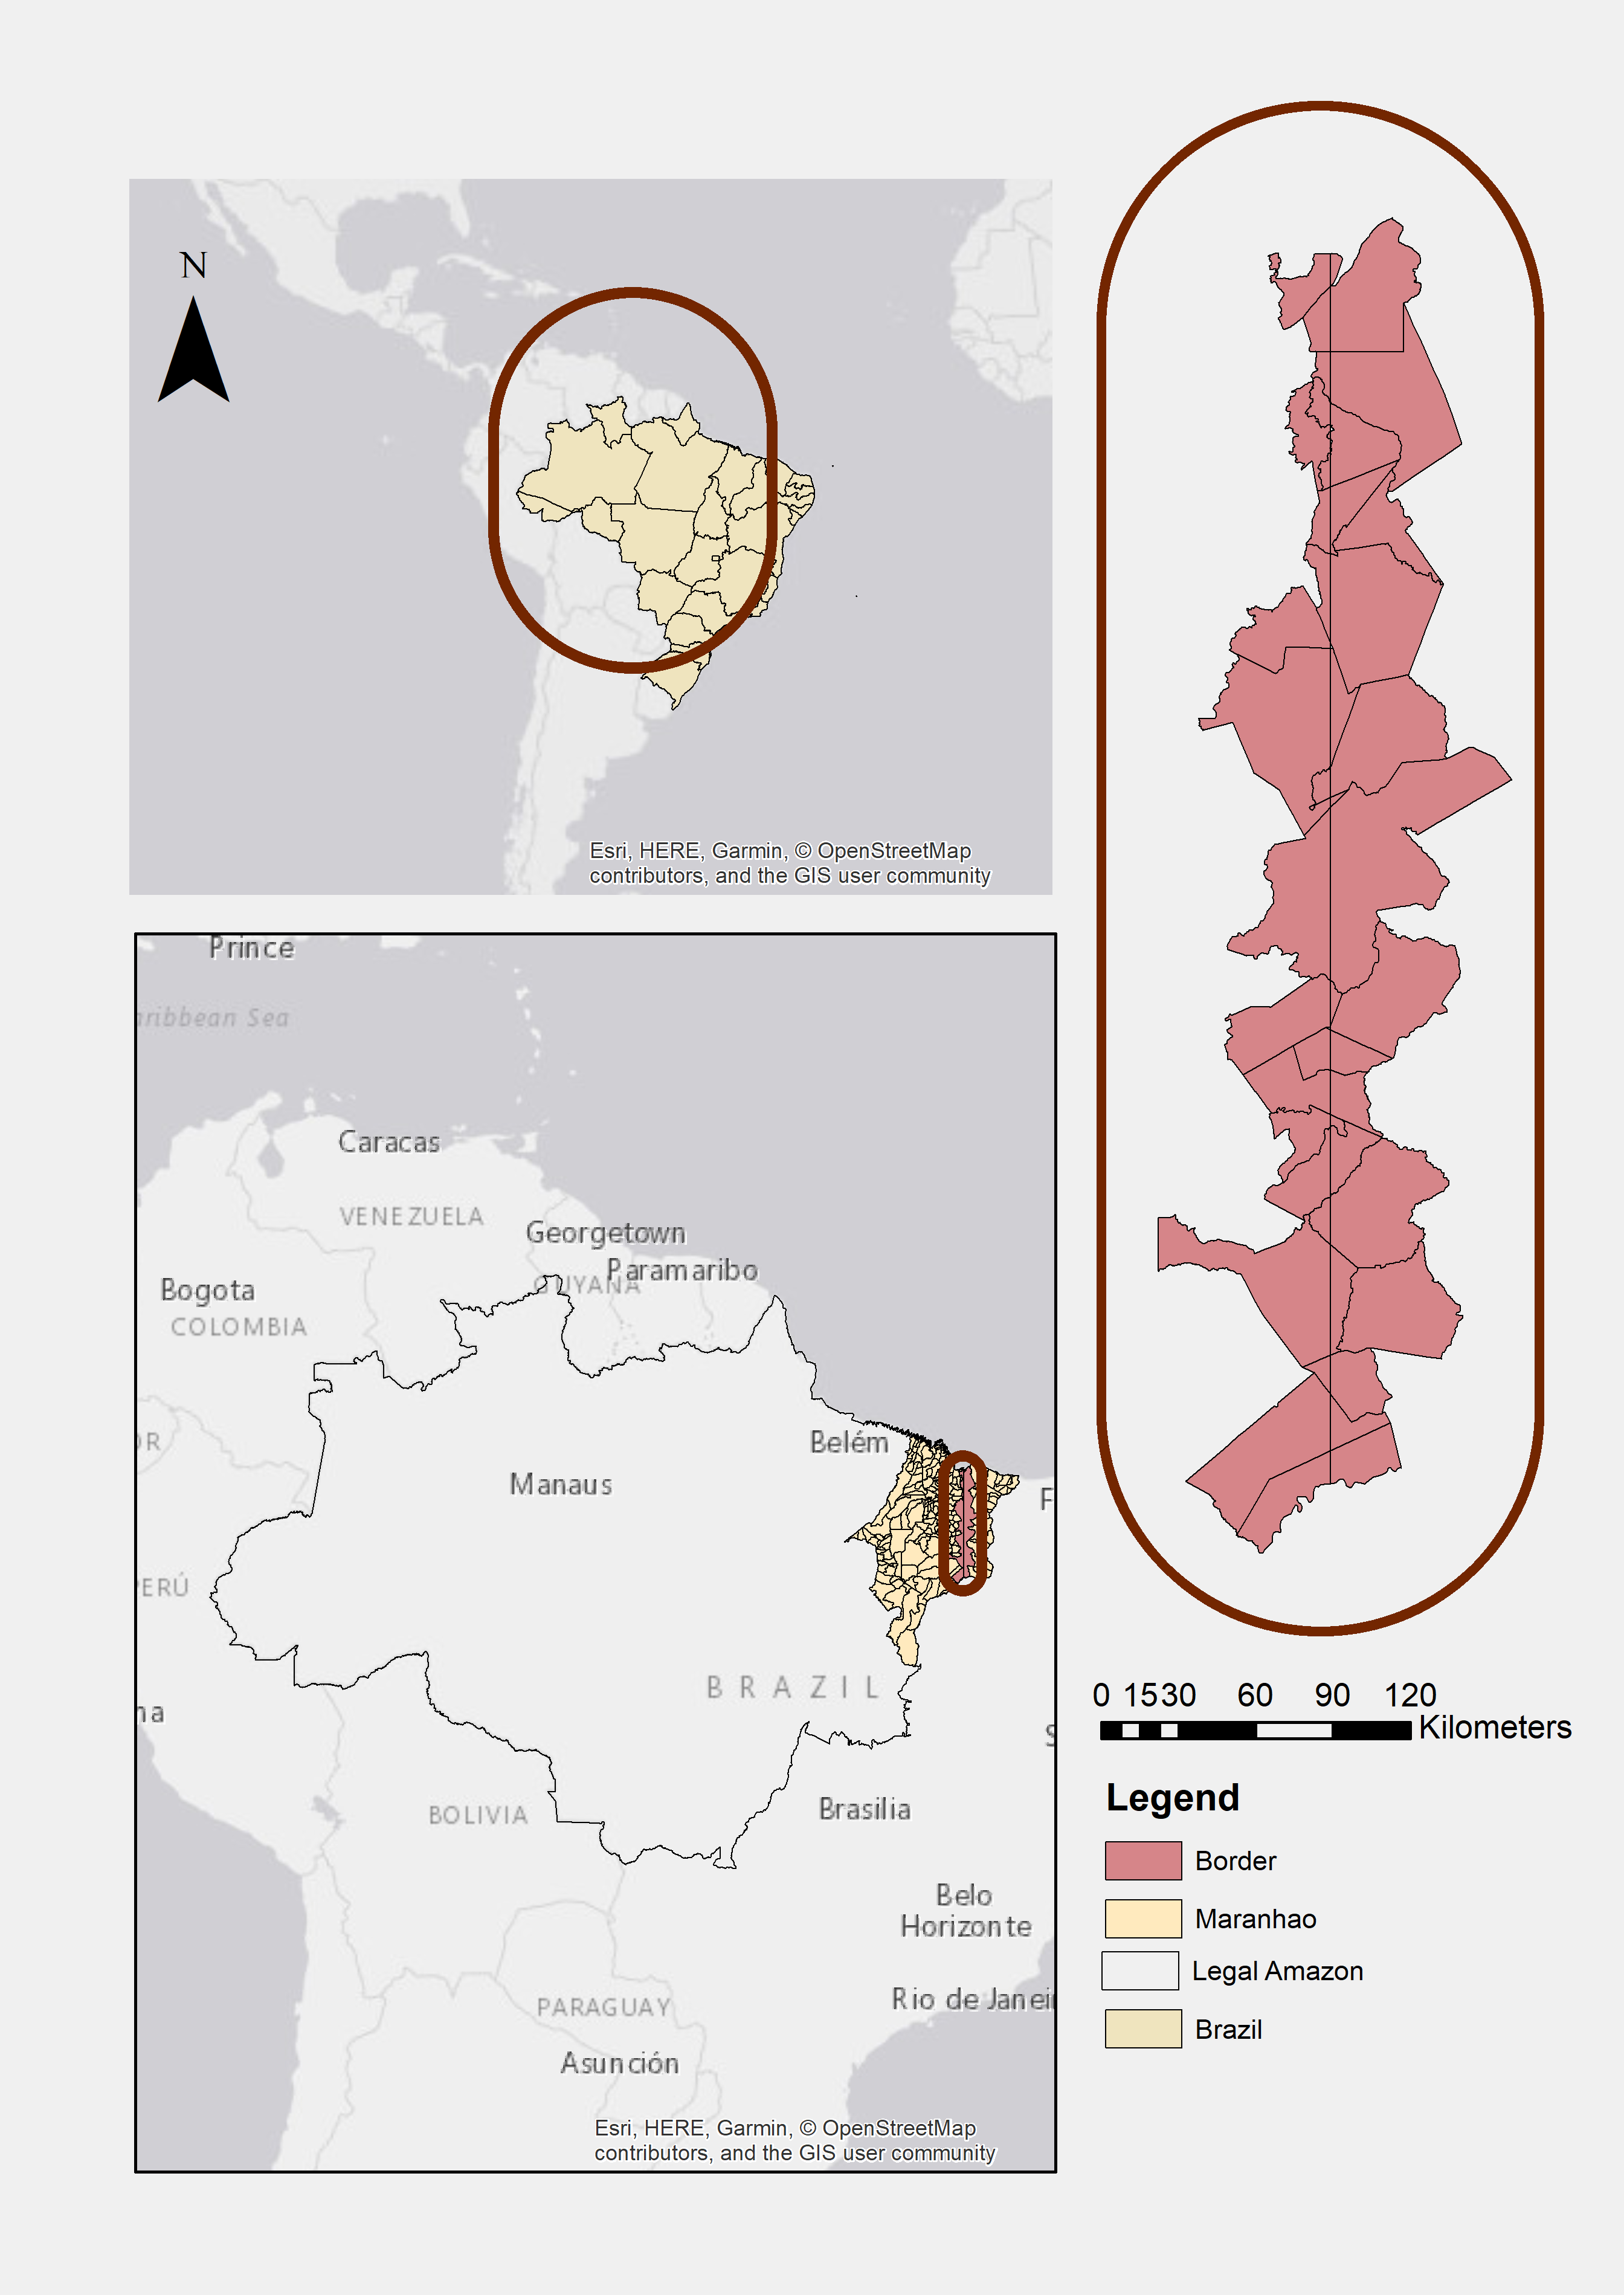
\includegraphics[width=1\textwidth, inner]{Chapter3/MaranhaoChapter3_Fig1.png}
\caption[Map of Maranhão Studied Area]{Map of Maranhão Studied Area. The vertical line in the Border refers to the artificial line that divides Legal Maranhão and Cerrado Maranhão. Source: \citep{MMMAwebsite,nugeo_2018}.}
\label{fig:delimitacao}
\end{figure}

%According to \citet{ferreira_2008, CELENTANO_2017, costa_2018}, recent forest losses in the studied region have been due to the creation of settlement projects, illegal logging, pasture, subsistence agriculture and commodities. During the 40's, Maranhão had more than 200,000 km$^{2}$ uninhabited land, which included transition forest, Cerrado, and pre-Amazon forest. The situation backed the creation of several settlement projects along with the creation of federal roads and the Carajas railway project.

%The site considered is of great uniqueness. The 21 municipalities are crossed by an imaginary line that divides these in two parts. The crossed area is homogeneous in several aspects such as biota, institutional framework, and, climate with the only difference being the surveillance environmental program that is observed in only one part of the municipality. To endorse our assumption, we calculate an effect size index for the two areas divided. Following \citet{COHEN1977}, we take differences of means expressed in terms of the pooled within areas standard deviation. The Index is interpreted in terms of the average percentile standing of one area relative to the other area. The test result shows an index of 0.2 which indicates that the mean of one area is at the 58th percentile of the buffer zone, i.e the dissimilarities for the two areas are close to zero.

\subsubsection{Environmental Policy: DETER monitoring system}

As noted previously, the PPCDAm policy has at its core two satellite-monitoring operating systems, the PRODES and DETER, which were designed to meet different objectives at different times. PRODES system measures annual clearing rates since 1988, for increments of over 6.25 hectares. Because it uses a fine resolution, it is more detailed and depends on the climatic conditions of the dry season for acquisition of cloud-free images. These images are obtained between May and September, and the deforestation rate is calculated once a year.

In contrast, DETER alerts are conducted for the purposes of support to inspection. The alerts are issued bi-weekly and sent to the environmental police (IBAMA) and to environmental agencies of the states of the Legal Amazon to plan their field actions and operations to combat illegal deforestation. For the general public, the alerts are combined into monthly reports for the period between May and October, when the cloud cover decreases and it becomes possible to observe the region relatively cloud free. During the period from November to April, when there is greater cloud cover, DETER's public reports are quarterly.

The real-time detection system identifies and maps deforested areas in forest formations in the Amazon. This system uses images from MODIS sensors, aboard NASA's TERRA satellite and WFI images aboard the Brazilian CBERS-2B satellite \citep{inpe-deter_2018}. These sensors cover the Amazon with high temporal frequency, of two and five days, respectively, but with limited spatial resolution of 250 meters and 260 meters (WFI). With this spatial resolution, the images allow the detection of deforestation the areas of which are greater than 250m (or 25 hectares). Since the satellite used in DETER is incapable of detecting land cover patterns in areas covered by clouds, no forest clearing activity is identified in these areas, and thus no alerts pinpointing the location of recent deforestation activity are issued for the region and time covered by clouds \citep{ASSUNCAO_2017}.

The high frequency of observation is one way to compensate for the limitation of the spatial resolution. Most importantly, the high frequency reduces the problems imposed by the frequent cloud cover in the Amazon region. In the Amazon forest, the cloud formation depends on the topography of the place. Usually at the north of Amazon forest there is more cloud persistence, and distance to water basin and the ocean matters, as normally cloud forms far from water reservoirs. \citet{Wang2004,Koren2004,Wang2009,Pinto2009,Heiblum2014} discovered that there is a relationship between cloud cover and land cover in Amazon forest. The evapotranspiration properties of the land cover vegetation are tightly linked to the dynamics of the boundary layer and the formation of clouds, which commonly cap the boundary layer. Deforested areas in the Amazon (either pasture or cropland) usually display higher sensible heat and lower latent heat fluxes in comparison with the forested areas, which in turn can enhance the growth of the boundary layer during the day and favour the formation of larger clouds, i.e. deforested areas enact the presence of clouds and it is difficult to disentangle whether cloud favours deforestation or deforestation favours the formation of clouds. 

In the present study this phenomenon does not seems to happen because there is no presence of dense forest our study area that could favour cloud formation over the surrounding forested areas or that could influence the clouds to other areas (deforested ones). The ecological tension zone allows the clouds to spread uniformly within the area which excludes the causal effect found by several studies. We hypothesise that cloud coverage limiting satellite visibility in the DETER monitoring system affects the enforcement of the environmental policy in the forest transition area of Maranhão.

\subsection{Image preparation}  %mudar o titutlo

%Aqui colocar, remote sensing, modis 
When considering vegetation mapping for forest cover loss and forest regrowth path, traditional methods such as field surveys are time consuming, date acquisition lagged, and generally too expensive. Over the past four decades, a feasible alternative considered by researchers and specialists is to apply remote sense technology and subsequent image analysis. More precisely, the use of satellite time series along with statistical analysis can be helpful in understanding the characteristics of vegetation dynamics. In this paper we use images derived from the MODIS sensors.\footnote{A detailed summary of satellites, sensors and databases relevant to vegetation can be found in \citet{horning_2010}.}

%For instance, in 1999, a group of researchers around the world created the Global Land Cover 2000 (GLC2000) project extracting data from 1-km SPOT4-VEGETATION  imagery.\footnote{For the dataset, see http://www-gvm.jrc.it/glc2000/} After two years, US-NASA  released the  database  of  global  MODIS  land  cover  based  on  monthly composites from MODIS sensor for the period between January  and  December  2001 \citep{xie_sha_yu_2008}.\footnote{For the dataset, see http://duckwater.bu.edu/lc/mod12q1.html}

%In general, the  selection of  images  acquired  by  adequate sensors is largely determined by the mapping objective and accuracy, the cost of images, the climate conditions, such as a cloud-free image, and the technical issues that arise from interpretation and suitability. 
Freely available and with high temporal resolution, the MODIS sensor has two instruments. The Terra satellite is on an AM overpass, whereas the Aqua platform provides complementary observations in the afternoon. The Terra orbital configuration and MODIS viewing geometry produce full global coverage every one to two days, except for the equatorial zone, where the repeat frequency is approximately 1.2 days \citep{zhan_2002, setiawan_2014}. The high temporal resolution of MODIS is a determining factor in phenological studies and spectral discrimination, and can be used to obtain detailed knowledge about the seasonal cycles of vegetation in biomes with strong seasonal contrast, such as the Cerrado biome and the Ecotone forest. An additional advantage of the MODIS data is that is in a ready-to-use format.

To derive our dataset we use two products created by MODIS sensor: MCD12Q1 and MOD13Q1. These products were retrieved from the online Application for Extracting and Exploring Analysis Ready Samples (AppEEARS) tool courtesy of the NASA EOSDIS Land Processes Distributed Active Archive Center (LP DAAC), USGS/Earth Resources Observation and Science (EROS) Center, Sioux Falls, South Dakota, \citep{didan_2015,didan_munoz_2015,sulla_2015,sulla2_2018}. The MODIS Land Cover Type Product (MCD12Q1) provides 13 science data sets (SDSs) that map global land cover at the 500m spatial resolution in annual time steps for six different land cover legends from 2001-2016 and includes 5 legacy classification schemes, such as the University of Maryland classification (UMD) (see Table \ref{UMD}), which recognises 17 classes, covering natural vegetation (11 classes), mosaic lands (2 classes), and non-vegetated lands (4 classes) \citep{setiawan_2014, friedl_2018}. 

\begin{table}[H]
\footnotesize
\caption{University of Maryland (UMD) legend and class definitions}
\begin{tabularx}{\linewidth}{X B X}
\hline
\hline
Name & Class & \centering\arraybackslash Description\\
\hline
Water	&	0	&	At least 60\% of area is covered by permanent water bodies	\\
Evergreen Needleleaf forest	&	1	&	Needleleaf Forests 1 Dominated by evergreen conifer trees (canopy >2m). Tree cover >60\%.	\\
Evergreen Broadleaf forest	&	2	&	Dominated by evergreen broadleaf and palmate trees (canopy >2m). Tree cover >60\%.	\\
Deciduous Needleleaf forest	&	3	&	Dominated by deciduous needleleaf (larch) trees (canopy >2m). Tree cover >60\%.	\\
Deciduous Broadleaf forest	&	4	&	Dominated by deciduous broadleaf trees (canopy >2m). Tree cover >60\%.	\\
Mixed forest	&	5	&	Dominated by neither deciduous nor evergreen (40-60\% of each) tree type (canopy >2m). Tree cover >60\%.	\\
Closed shrublands	&	6	&	Dominated by woody perennials (1-2m height) >60\% cover.	\\
Open shrublands	&	7	&	 Dominated by woody perennials (1-2m height) 10-60\% cover.	\\
Woody savannas	&	8	&	Tree cover 30-60\% (canopy >2m).	\\
Savannas	&	9	&	Tree cover 10-30\% (canopy >2m).	\\
Grasslands	&	10	&	 Dominated by herbaceous annuals (<2m).	\\
Permanent Wetlands	&	11	&	Permanently inundated lands with 30-60\% water cover and >10\% vegetated cover.	\\
Croplands	&	12	&	At least 60\% of area is cultivated cropland.	\\
Urban and built-up	&	13	&	At least 30\% impervious surface area including building materials, asphalt, and vehicles.	\\
Cropland/Natural Vegetation Mosaics	&	14	&	Mosaics of small-scale cultivation 40-60\% with natural tree, shrub, or herbaceous vegetation	\\
Non-Vegetated Land	&	15	&	At least 60\% of area is non-vegetated barren (sand, rock, soil) or permanent snow and ice with less than 10\% vegetation.	\\
Unclassified	&	255	&	 Has not received a map label because of missing inputs	\\
\hline
\hline
\multicolumn{3}{l}{\footnotesize  Note: Source: \cite{sulla2_2018}.}
\end{tabularx}
\label{UMD}
\end{table}


The MODIS Vegetation Indices (VI) (MOD13Q1) product consists of time series comparisons of global vegetation conditions that can be used to monitor the Earth's terrestrial change detection. The two vegetation indices that we derive from these are the Normalized Difference Vegetation Index (NDVI) and the Enhanced Vegetation Index (EVI). The NDVI is a normalized transformation of the NIR (Near Infrared) and red reflectance ratio standardized to range from -1 to 1. The EVI is an optimisation of the vegetational signal that minimises noise, and has been reported to be more responsive to canopy structural variations, including canopy type. The EVI formula is written as: 

\setlength{\belowdisplayskip}{0pt} \setlength{\belowdisplayshortskip}{0pt}
\setlength{\abovedisplayskip}{0pt} \setlength{\abovedisplayshortskip}{0pt}

%COLOCAR AQUI A EQUACAO DO EVI
\begin{center}
\begin{equation}
EVI = \frac{\rho_{NIR} - \rho_{red}}{\rho_{NIR} + C_{1\rho_{red}} - C_{2\rho_{blue}} + L} (G) \label{eq:2} 
\end{equation}
\end{center}

where $\rho_{red}$ and $\rho_{NIR}$ and $\rho_{blue}$ are the reflectance in MODIS bands 1,2 and 3 (459-479nm) and C$_{1}$ and C$_{2}$ are the atmospheric resistance coefficients. L and G are the canopy background adjustment and the gain factor, respectively. The coefficients adopted for the MODIS EVI algorithm are L=1, C$_{1}$ =6, C$_{2}$ =7.5, and G=2.5. The EVI differs from NDVI by attempting to correct for atmospheric and background effects. In addition, EVI is superior in discriminating subtle differences in areas of high vegetation density than NDVI because the latter tends to saturate \citep{didan_munoz_2015, ratana_huete_ferreira_2005}. The NDVI takes the form of:


%COLOCAR AQUI A EQUACAO DO NDVI
\begin{center}
\begin{equation}
NDVI = \frac{\rho_{NIR} - \rho_{red}}{\rho_{NIR} + \rho_{red}} \label{eq:1} 
\end{equation}
\end{center}

where $\rho_{red}$ and $\rho_{NIR}$ are the surface bidirectional reflectance factors for MODIS bands 1 (620-670nm) and 2 (841-876nm). 

To construct our forest survival dataset we collected the 16-days-250m image from the first period and compared it to the 16-days image from the second period of the same month. First, we used two masks in the analysis, namely the Goodness of Fit mask and Land Cover mask. The Goodness mask was used to filter pixels flagged with bad quality. For the Land Mask, we resampled the rasters to 250m and applied the mask to differentiate pixels from land, forest, built-in and water. Through comparison it was possible to detect if the pixel with NDVI and EVI values survived from period one to period two within the month. This approach was undertaken for all the images corresponding to NDVI and EVI values for each 2 periods of the month of each year, which corresponds to 776 image analyses. For the leap years process we stopped at the land cover mask filtering process and we used the first period of 16-days as the main period. To compose the dataset we created a Boolean list of every image acknowledging if the pixel survived during that period or not, then we aggregated the list to year periods and computed the corresponding year of deforestation. To determine if the pixel survived, we used the rules outlined in Table \ref{assumption}. At the end of the process pixels were selected within the area studied (see Figure \ref{fig:delimitacao}), and measured in distance from the artificial Legal Amazon line to the west and east portions of the municipalities. When the pixel had a variation greater than 0.1 within a month, it was labelled as a disturbance. Any disturbances below 0.1 are considered measurement error.  Disturbances greater than 0.1 that result in negative changes in vegetation indices are considered as at least some deforestation having taken place in that pixel.  We do not re-examine the pixel once it has been identified as having been deforested.  With the identification of the time point of deforestation of a pixel we calculate the time of survival as the time since the beginning of our sample period. As a demonstrative example, we show the remaining pixels in the Legal Maranhão (LM) and Cerrado Maranhão (see Figures \ref{fig:remainingLM} and \ref{fig:remainingMA}).  

\begin{table}[H]
\footnotesize
\caption{Algorithm Assumption for NDVI and EVI values}
\begin{tabularx}{\linewidth}{X X X}
\hline
\hline
$NDVI_{1} > NDVI_{2}$	& ->  $NDVI_{1} - NDVI_{2}$	 & Numbers (1) and (2) refer to the order of the period of the month \\
$NDVI_{1} <= NDVI_{2}$	& ->  $NDVI_{1} = NDVI_{2}$	 & Numbers (1) and (2) refer to the order of the period of the month. The second equation assumes that values did not change within the month and then the value assigned is from the last observation	\\
\hline
$EVI_{1} > EVI_{2}$	& ->  $EVI_{1} - EVI_{2}$	 & Numbers (1) and (2) refer to the order of the period of the month \\
$EVI_{1} <= EVI_{2}$	& ->  $EVI_{1} = EVI_{2}$	 & Numbers (1) and (2) refer to the order of the period of the month. The second equation assumes that values did not change within the month and then the value assigned is from the last observation 	\\
\hline
\hline
\end{tabularx}
\label{assumption}
\end{table}

To obtain the cloud cover dataset we first used the Goodness mask to create an image from the 16-days first and second periods containing only pixels flagged with clouds. After creating the image for a month, we summed all month images in order to have the number of months that a pixel with a cloud upon it. With these we performed a Kernel Regression of the share of deforested pixels on the number of periods with cloud cover to check the threshold period for cloud cover persistence. To this end we used the optimal bandwidth suggested by \citet{bowman_azzalini_1997} with 1000 replications with cross-validation. This suggested a threshold of about 9 months. With the identified threshold, we applied a third mask called Cloud Mask to all the images processed of each year before conducting the Boolean List. If within a year the pixel was equal to or exceeded the threshold, then it was flagged as a cloud persistence pixel; See algorithm implementation in \ref{fig:method} for details. While this decision rule will inevitable identify some pixels as clouded after their deforestation, excluding them does not change our results in any noticeable manner. \footnote{We ran regressions taking into consideration pixels presenting cloud cover before deforestation and the results don't change from what we are presenting in this chapter.}


%Colocar sobre as covariates ou risk factors

The risk factor (covariate) variables were acquired in shapefile format from different sources (see Table \ref{tab:sources}). To get the distance from each pixel to the covariates we transformed the files into raster format and performed an Euclidean distance calculation from each pixel to the variable source within the studied area. The source variables were roads, protected areas, indigenous land, markets, municipalities centre, and, mining/mineral resources existent before or from 2000. For rivers, latitude, longitude, and elevation we simply used the distance to them. Time dependent variables were partitioned into five year averages in order to make their computation feasible. More precisely we calculated 5-year measures of neighbouring forested pixels and average levels of rainfall and temperature for the years 2001, 2006, 2011 and, 2016. 

\subsection{Survival Models}  %mudar o titutlo

Survival analysis is a statistical method designed to study the amount of time an experimental unit survives. Originally, the event of interest was mortality and the analysis consisted of following the subjects until death. In recent years, the identification of risk and/or prognostic factors related to survival have been applied much more widely.  What distinguishes survival analysis from other areas in statistics is that survival data are usually censored \citep{lee_wang_2003,cao_2005}. The defining feature of censored data is that the event time of interest is not always fully observed on all subjects under study. We consider three survival approaches in this study: the Kaplan Meier (KM) model,  the Cox Proportional Hazard model (CPH), and the Extended Cox Proportional Hazard model (ECPH).

%Colocar a explicacao do KM

Let \textit{n} be the total number of pixels of NDVI and EVI values whose survival times, censored or not, are available. Relabel the n survival times in order of increasing magnitude. Then

\begin{center}
\begin{equation}
\hat{S}(t) = \prod_{t_{(r)} \leq t} \frac{n-r}{n-r + 1}\label{eq:3} 
\end{equation}
\end{center}

where \textit{r} runs through those positive integers for which $t_{(r)} \leq t$ and $t_{(r)}$ is not censored. The values of \textit{r} are consecutive integers 1, 2,\dots , n if there are no censored observations; if there are censored observations, they are not. The estimated median survival time is the 50th percentile, which is the value of $t$ at $\hat{S}(t)$ = 0.5. More precisely, it is a step function, and is the nonparametric maximum-likelihood estimator of the product limit estimates proposed by Kaplan and Meier \citep{lee_wang_2003}.


%Colocar a explicacao do Cox Proportional

Extending the analysis to the inclusion of risk factors and time dependent variables, the most common approach used is the Cox Proportional Hazard model which can handle censored and/or truncated observations \citep{Cox1972,cao_2005}. 

Again, let \textit{n} be the total number of pixels of NDVI and EVI values which consists of $t_{(j)}$, $\delta_{(j)}$, $z_{(j)}$, $\textit{j}$ = 1,2,\dots,\textit{n}, where $t_{(j)}$ is
the time under study for the \textit{j}th pixel, $\delta_{(j)}$ is the deforestation indicator ($\delta_{(j)}$ = 1 if the deforestation has occurred and $\delta_{(j)}$ = 0 if the pixel is right-censored), and $z_{(j)}$ is the vector of risk factor for the \textit{j}th pixel that may affect the distribution of \textit{X}, the time to deforest.

Let $h(t|z)$ be the hazard rate in the sub population with covariate value(s) z. The Cox proportional hazards regression model relates covariates to the hazard function as follows:

\begin{center}
\begin{equation}
h(t|z) = h_{0}(t)c(\beta^{'}z) \label{eq:4} 
\end{equation}
\end{center}

where $h_{0}(t)c(0)$ is the hazard function for the sub population with covariate value z = 0 and is called the baseline hazard function, $\beta$ = ($\beta_{1}$,$\beta_{2}$,\dots, $\beta_{p}$) is a parameter vector of regression coefficients, $\beta^{'}z = \sum^{p}_{i=1}\beta_{k}z_{k}$, and $c(.)$ is a fixed, known scalar function. This model is semi-parametric because the baseline hazard model is estimated non parametrically, while the risk factors are constrained by the parametric representation $c(\beta^{'}z)$. The parametric function usually assumes the exponential form 


\begin{center}
\begin{equation}
c(\beta^{'}z) = exp(\beta^{'}z) = exp(\sum^{p}_{k=1}=\beta_{k}z_{k}) = e^{\sum^{p}_{k=1}=\beta_{k}z_{k}}  \label{eq:5} 
\end{equation}
\end{center}

where 

\begin{center}
\begin{equation}
h(t|z) = h_{0}(t)c(\beta^{'}z) = h_{0}(t) exp(\sum^{p}_{k=1}=\beta_{k}z_{k}) \label{eq:6} 
\end{equation}
\end{center}

The Cox model is often called a proportional hazards model because, if we look at two pixels with covariate values $z_{1}$ and $z_{2}$, the ratio of their hazard functions at time \textit{t} does not depend on \textit{t} and the hazard rates are proportional \citep{cao_2005}.

\begin{center}
\begin{equation}
\frac{h(t|z_{1}) = h_{0}(t)exp(\beta^{'}z_{1})}{h(t|z_{2}) = h_{0}(t)exp(\beta^{'}z_{2})} = exp[(\beta^{'}(z_{1} - z_{2}))]  \label{eq:7} 
\end{equation}
\end{center}


%Colocar a explicacao do KM, Cox Proportional e com o Time dependent
An issue might arise from the possibility of unobserved heterogeneity (spatial and temporal dimensions) that would result from a misspecification of the survival model. To control for these two types, we include the 5-year averages of the share of neighbouring pixels with forest remaining, rainfall, and temperature. Extending the Cox Proportional Hazard model by adding a time dependent variable, the basic model is done by replacing z by z(t) ($T_{(j)}$, $\delta_{(j)}$, [$z_{(j)}(t), 0 \leq t \leq T_{j}$]), so that


\begin{center}
\begin{equation}
h(t|z_{s}, 0 \leq s \leq t) = h_{0}(t)exp[\sum^{p}_{k=1}\beta_{k}z_{k}(t)] \label{eq:8} 
\end{equation}
\end{center}

where $T_{j}$ is time on study for the \textit{j}th pixel, and $\delta_{(j)}$ the deforestation event for the \textit{j}th pixel ($\delta_{(j)}$ = 1 if deforestation has occurred and, $\delta_{(j)}$ = 0 if the pixel was not deforested during the period (right-censored)). In addition, $z_{(j)}(t)$ corresponds to the vector of risk factors for the  \textit{j}th pixel which includes measures of elevation, and distance to rivers, mining, roads, markets, municipality centres, protected areas and, cloud persistence. We interact some of the controls and risk factors with a region dummy (Legal Maranhão = 1 and Cerrado Maranhão = 0).

\subsubsection{Data Analysis}  %mudar o titutlo
An important assumption of our analysis is that the two buffer zones that we created around the artificial line to isolate and compare pixels, are homogeneous biologically. To find further support for this we first calculated an effect size index for the two areas divided. Following \citet{COHEN1977}, we take differences of means expressed in terms of the pooled within areas standard deviation. The Index is interpreted in terms of the average percentile standing of one area relative to the other area. The test result shows an index of 0.2 which indicates that the mean of one area is at the 58th percentile of the buffer zone, i.e the dissimilarities for the two areas are close to zero.  Since the chosen buffer zone may seem somewhat arbitrary, we also examined whether forests between the two regions differ right outside the buffer zone.  More precisely, we isolated the areas 0.2 degrees just outside buffer zone on each side of the two regions and similarly tested their difference.  The corresponding Cohen index was 0.59, which is at the 69th percentile,  and thus one can reject the null hypothesis that there is no difference between these two regions. As a matter of fact, the index value of 0.59 indicates a distinction of 33\% in the two distributions \citep{COHEN1977}.


The non parametric and semi parametric models presented in this study are estimated using MODIS satellite derived data as the dependent variable and several biophysical, economic and environmental spatial data for the covariates. Table \ref{tab:summary} provides the summary statistics for our response and risk factors variables and Table \ref{tab:sources} provides the variables' sources. Our sample contains approximately 530,000 observations (for the combined MA and LM region) with the time each pixel was deforested as well as eight influencing risk factors and several controls.

Overall, the average time a pixel in our sample becomes deforested is 2.6 years for NDVI values and 2.4 years for EVI values. Note that nearly 71\% of the pixels are covered by clouds and that the average distance to protected areas is about 58 km$^{2}$ for the studied area. Markets, municipalities and roads have an average distance of 55 , 13,  and 4 km$^{2}$, respectively. The region is extensively surrounded by rivers to which the average distance is less than 2 km$^{2}$. Particularly in the region of Maranhão there is a high concentration of mineral resources, where the average distance between the pixels and mines is equivalent to approximately 6 km$^{2}$. In addition, 40\% of the pixels belong to the LM region and almost 97\% of the analysed pixels were at some time deforested.

%colocar sobre validation dos resultados k-fold e concordance index
To conduct the analysis, we extensively used Python and R language and specific packages and modules, such as lifelines from \citet{cameron_2018} and survival from \citet{survival-book,survival-package}. In survival analysis with censorship it is not appropriate to use a loss function like mean-squared-error or mean-absolute-loss. Instead, we use the concordance-index, also known as the c-index. This measure evaluates the accuracy of the ordering of predicted time. It is in fact a generalization of the AUC (area under the curve), another common loss function, and is interpreted similarly \citep{cameron_2018}. More precisely, if the c-index has a value around 0.5, then it corresponds to the expected result from random predictions, whereas 1.0 is perfect concordance and 0.0 is perfect anti-concordance. Usually, survival models range from 0.5 to 0.7.

To validate the results, we perform k-fold validations. This entails splitting a training set from the data into k smaller sets (k=3, as default). A model is trained using $k-1$ of the folds as training data. The resulting model is validated on the remainder of the data, i.e., it is used as a test set to compute a performance measure such as accuracy. The performance measure reported by k-fold cross-validation is then the average of the values computed in the loop and should be close to 0 \citep{scikit-learn}. The c-index and k-fold validation results are computed in Table \ref{kfold}. As a further validation process we compute variable importance with p-values for high dimensional data. For this task we applied random forests classification. This testing approach is based on a modified version of the permutation variable importance, which is inspired by cross-validation procedures \citep{Janitza2016}. With an unbiased variable importance measure, the importance values of non-associated variables vary randomly around zero. Thus, all non-positive importance values are assumed to correspond to these non-associated variables and are used to construct a distribution of the importance under the null hypothesis of no association to the response. Since only the non-positive values of this distribution can be observed, the positive values are created by mirroring the negative distribution. We calculated less than 250 permutations and added 1 to the numerator and denominator to avoid zero p-values \citep{ranger_2018}. The results indicated that all variables are important to the model and, hierarchically, clouds, rivers, and roads are the most important measure in the model.

Statistical validation included several tests on non parametric and semi parametric fitters. For the KM estimator we conducted two different logrank tests. For the Cox proportional Hazard method we conducted Likelihood ratio, Wald, and score tests. All models showed good tests results rejecting the null hypothesis decisively. 

\section{Results}  %mudar o titutlo
\label{S:3}
We first examine the non parametric estimation of \citet{kaplanandmeier} of deforestation using NDVI and EVI values applied to the two regions (LM and MA) distinguished by the Legal Amazon line.  We secondly implement the semi parametric proportional hazard model proposed by \citet{Cox1972} and, as an extension, the extended proportional hazard model with time dependent variables. The results from the semi parametric analysis uses NDVI values because these responded better to our validation process\footnote{Results from EVI values do not differ from the results presented here. The suitability of the vegetational index is based on validation process.}.


\subsection{Non parametric Analysis} \label{resultssection1}
%MA + ML and %Log Rank test on Regions
As can be seen from Figure \ref{fig:km-total}, the chance of survival of the forests through the analysis of pixels was higher in the Cerrado Maranhão (MA) than in Legal Maranhão (LM). For the 529,680 pixel analysis, the rate of survival is lower for EVI values in all settings. In 2001 the rate of survival for EVI pixels in the whole region was about 59\% as compared to 61\% for NDVI pixels, but by  2010, the rate of survival decreased to 2\% and 3.2\%, respectively (see Table \ref{tab:KM_estimate}). The Log Rank test and Weighted Log Rank test confirms that the stratified samples differ in terms of distributions. 

\begin{figure}[H]
  \centering
  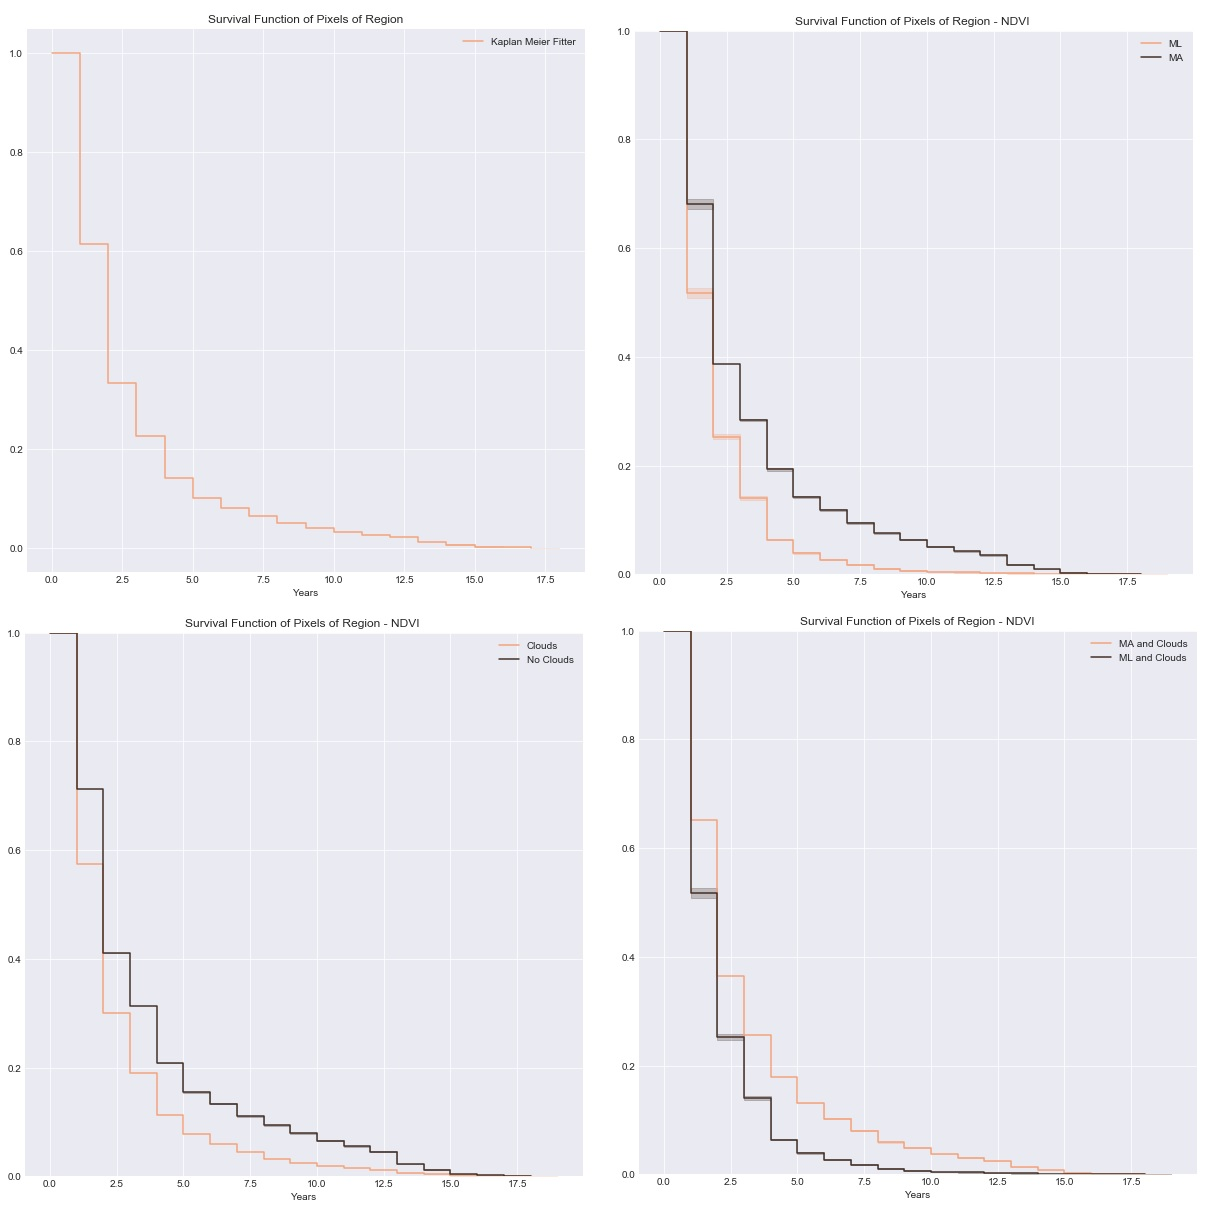
\includegraphics[width=1\textwidth]{KM_NDVI_complete.jpg}
\caption[Kaplan Meier Fitter for NDVI values in the complete Region ]{Kaplan Meier Fitter for NDVI values in the complete Region (LM+MA). Top left shows the KM fitter for the Region and, at the top right, the stratified KM fitter of the Region. Bottom left shows the KM fitter for the Region stratifying by cloud coverage. At the bottom right, it shows the KM fitter stratifying by Clouds and Region.}
\label{fig:km-total}
\end{figure}

\begin{table}[H]
\footnotesize
\caption{Kaplan Meier Estimation}
\begin{tabularx}{\linewidth}{l XXXXXX}
\hline
\hline
Time	&	Numbers at risk	&	Number of events	&	Survival 	&	Standard Errors  & lower 95\% CI & upper 95\% CI \\
\hline
Region  &&&&&& \\	
2001	&	512017	&	197454	&	0.61436	&	6.80E-04	&	0.61303	&	0.6157	\\
2005	&	71707	&	263281	&	0.10016	&	4.20E-04	&	0.09934	&	0.10098	\\
2011	&	20594	&	34998	&	0.0318	&	2.45E-04	&	0.03133	&	0.03229	\\
2015	&	3189	&	15180	&	0.00216	&	6.48E-05	&	0.00203	&	0.00229	\\
\hline
Region MA &&&&&& \\												\\
2001	&	302075	&	96251	&	0.68137	&	0.000848	&	0.6797	&	0.683	\\
2005	&	58271	&	162794	&	0.14245	&	0.000636	&	0.1412	&	0.1437	\\
2011	&	19179	&	27662	&	0.05087	&	0.0004	&	0.0501	&	0.0517	\\
2015	&	2946	&	14404	&	0.00319	&	0.000103	&	0.003	&	0.0034	\\
\hline
Region LM &&&&&& \\												\\
2001	&	209942	&	101203	&	0.517948	&	1.09E-03	&	0.515815	&	0.52009	\\
2005	&	13436	&	100487	&	0.039306	&	4.24E-04	&	0.038484	&	0.040146	\\
2011	&	1415	&	7336	&	0.004363	&	1.44E-04	&	0.00409	&	0.004654\\
2015	&	243	&	776	&	0.000667	&	5.63E-05	&	0.000565	&	0.000787\\
\hline
\hline
\end{tabularx}%
\label{tab:KM_estimate}%
\end{table}%

%MA
For the Cerrado Maranhão (MA), the Kaplan Meier fitter shows that from the 315,904  forested pixels in 2001, between 64\% to 68\%  had a chance of survival considering both vegetation indices. By 2010 this decreased to a range of 3\% to 5\%. At the end of our sample period, the chance of survival for pixels within Cerrado Maranhão was around 0.3\% (see upper left graph from Figure \ref{fig:km-evi} and Figure \ref{fig:km-ndvi}) and Table \ref{tab:KM_estimate}. The median time of survival for the model was two years. This means that the half life of the sample pixels was around two years (the 50th percentile).

%MA + clouds 

In calculating the survival curves by the presence of clouds one discovers that pixels with no clouds over the studied period had a higher rate of survival comparing to pixels with clouds. At the end of 2001, the rate of survival for pixels with no clouds was about 66.6\% to 71.2\% for both indices. In 2005, the rate lowered to around 15\% and, in 2015, the chance of survival of the forests was approximately 0.4\%. Looking at the survival curve of pixels covered by clouds, the chance of forest survival in 2001 was around 61\% to 65\%, then decreased to between 11\% and 13\% in 2005. The rate of survival for forests by 2015 was around 0.2\% for both vegetation indices (see upper right graph from Figure \ref{fig:km-evi} and Figure \ref{fig:km-ndvi} ). The median time of survival for the survival curves stratified by clouds did not change from the original set. 


%Log Rank test on MA clouds
We conducted a Log Rank test \citep{Peto_1972} to check whether the sub samples by cloud coverage were originated from the same distribution. The results showed that, in fact, these sub samples come from significantly different distributions. Since the majority of the pixels are deforested within two years, we also applied the generalized Wilcoxon test, also referred to as the Log Rank Weighted test because it gives more weight to earlier deforestation than later deforestation observations, while the Log Rank test gives equal weight to the whole deforestation process \citep{lee_wang_2003}. The results reinforce the earlier findings that the two survival curves are different from each other.

%ML + %ML + clouds
The Legal Maranhão (LM) experienced a similar pattern in that the median time of survival of the pixels was two years. From the 213,776 pixels analysed, approximately 51\% of the total had a chance of survival in 2001. This rate drops to about 4\% in 2005 and ten years later to 0.06\%. As apparent from the survival curve, the rate of survival was lower for the Legal Maranhão (LM). Stratifying by cloud coverage, the survival curves show that pixels without the presence of clouds had a higher rate of survival for both indices (see lower right graph from Figure \ref{fig:km-evi} and Figure \ref{fig:km-ndvi}). The rate of survival for pixels with no clouds was about 58.8\% to 59.2\% in 2001. then dropped to around 2.5\% in 2010, and was reduced to a zero rate of survival of pixels by 2015. The chance of survival for pixels covered by clouds was around 51\% in 2001 for both indices, i.e., almost 10\% lower when compared to non-clouded pixels. In 2010, the rate of survival was less than 0.5\% and in 2015 was equivalent to 0.065\%. 

%Log Rank test on ML clouds
We performed a Log Rank test \citep{Peto_1972} to check whether the two sub samples originated from the same distribution and the differences from these survival curves were due to other characteristics than the presence of clouds. The test result showed that the two sub samples are from different distributions. We was also applied the generalized Wilcoxon test \citep{lee_wang_2003} which rejected the null hypothesis that the two series came from the same distributional origin. 

\begin{figure}[H]
  \centering
  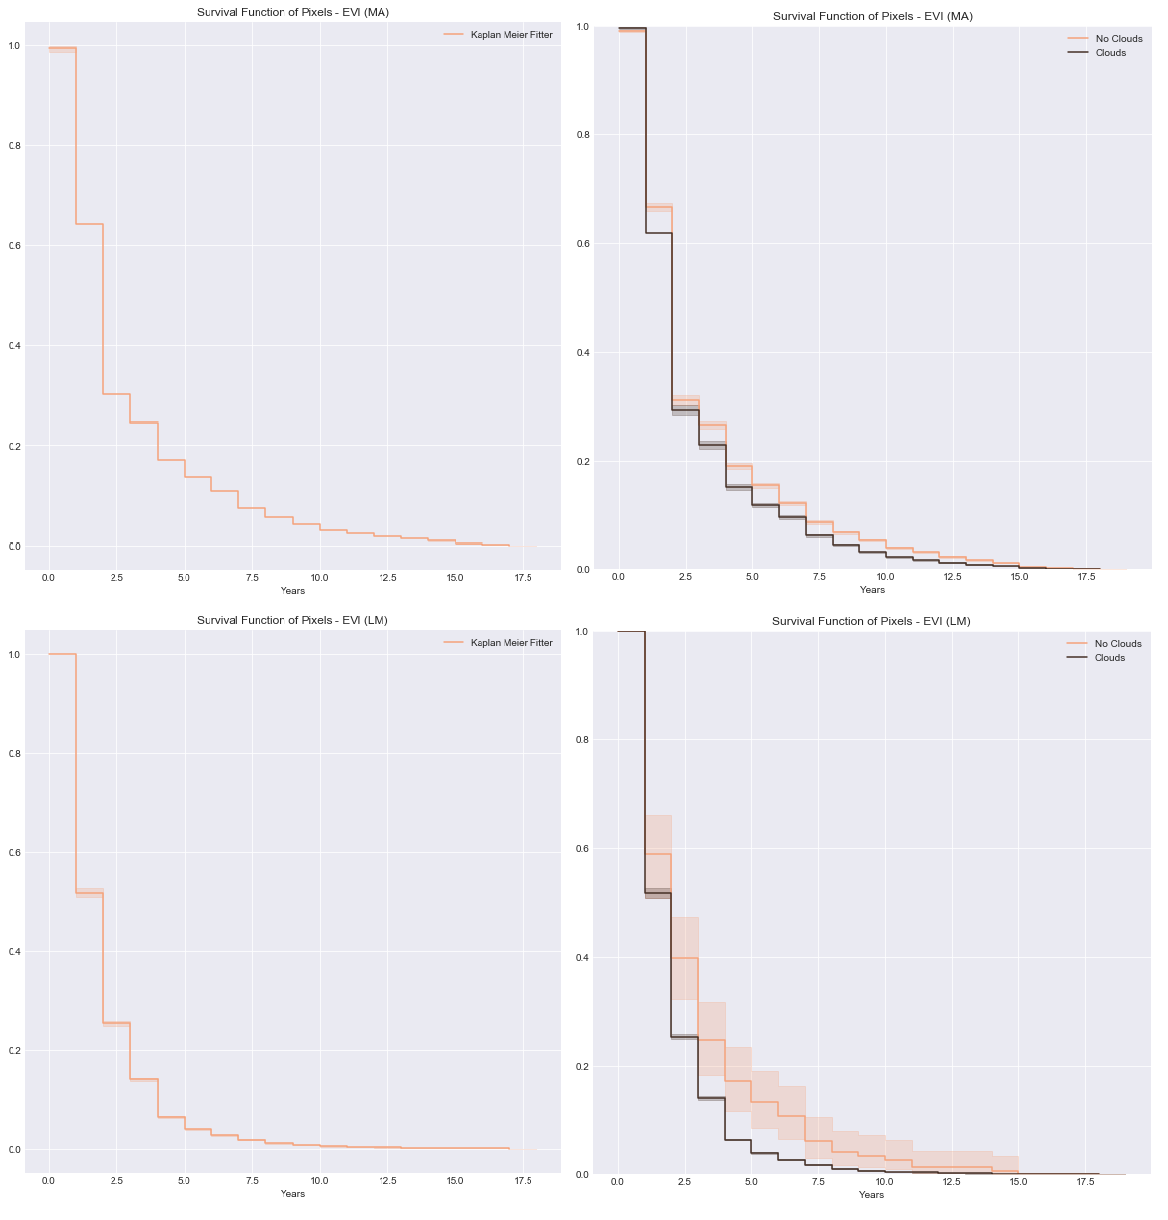
\includegraphics[width=1\textwidth]{KM_EVI.png}
\caption[Kaplan Meier Fitter for EVI values in LM and MA region separately.]{Kaplan Meier Fitter for EVI values in LM and MA region separately. Top left and right show the KM fitter for the Cerrado Maranhão  and, at the bottom, for the Legal Maranhão . The top and bottom left show the sides KM fitter. The top right and bottom show the sample stratified by cloud coverage. The coloured band represents 99\% confidence interval.}
\label{fig:km-evi}
\end{figure}

\begin{figure}[H]
  \centering
  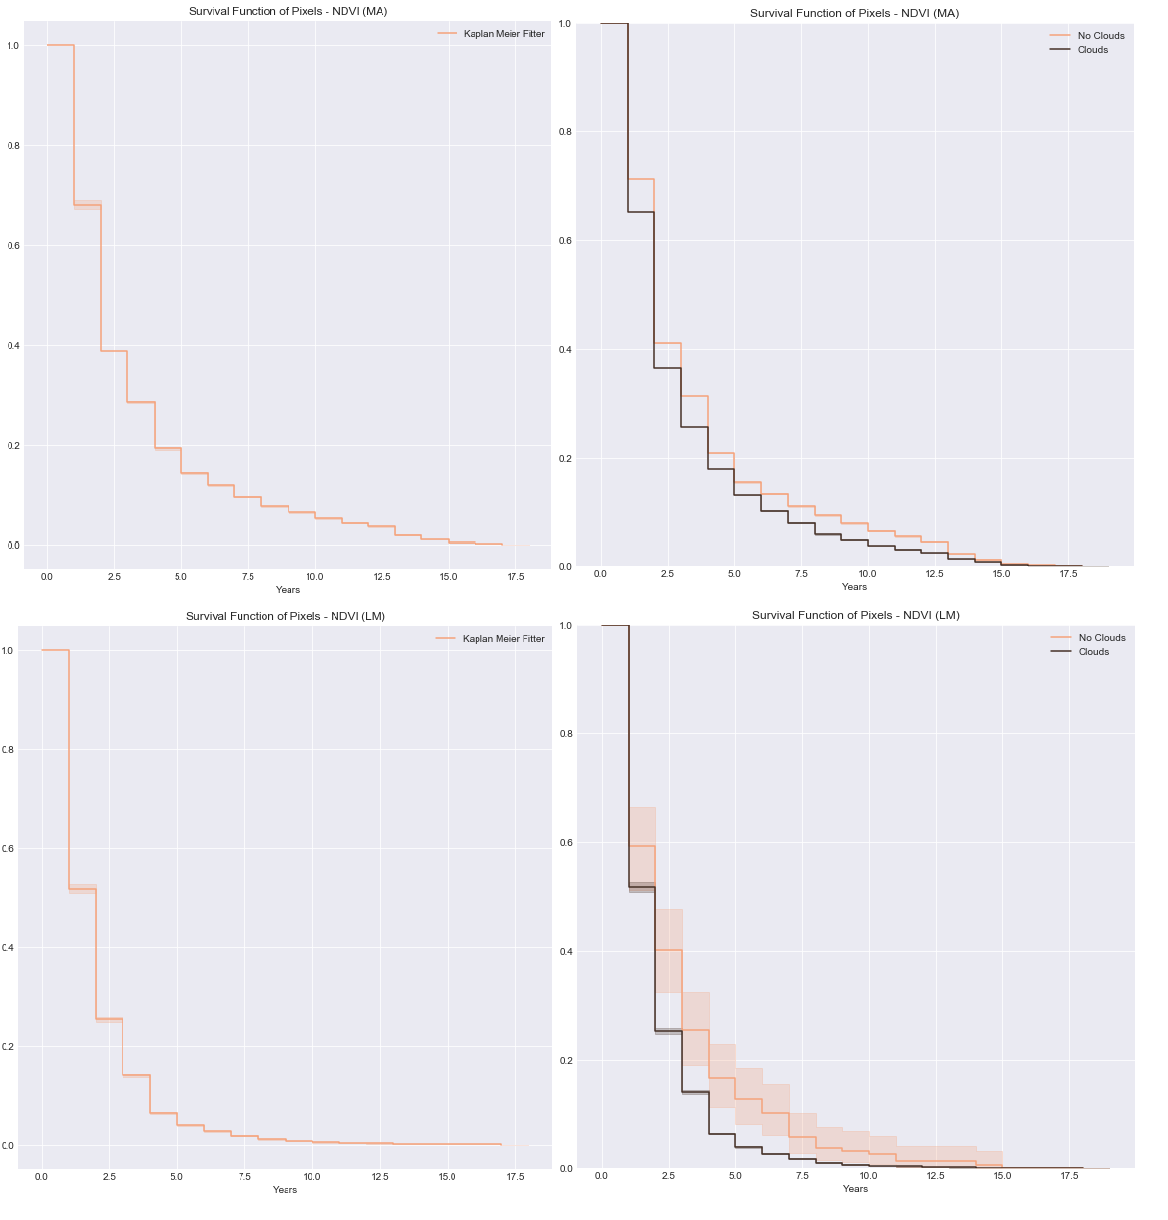
\includegraphics[width=1\textwidth]{KM_NDVI.png}
\caption[Kaplan Meier Fitter for NDVI values in LM and MA region separately.]{Kaplan Meier Fitter for NDVI values in LM and MA region separately. Top left and right show the KM fitter for the Cerrado Maranhão  and, at the bottom, for the Legal Maranhão . The top and bottom left show the sides KM fitter. The top right and bottom show the sample stratified by cloud coverage. The coloured band represents 99\% confidence interval.}
\label{fig:km-ndvi}
\end{figure}


\subsection{Semi parametric Analysis} \label{resultssection2}

%MA + ML
Studying forest loss and, in consequence, deforestation reveals that many factors potentially affect the process. In this sense, we expand the analysis to include risk factors (covariates) to evaluate the effect of these variables on forest survival (see \ref{eq:6}). 

We first start off by pooling the data across the two regions of interest.  In this regard, the preferred model was the NDVI model considering the concordance index (0.755) and k-fold model validation (0.03). We also checked the proportional hazard assumption with plots of each estimated regression coefficient as a function of time through the smoothed scaled Schoenfeld residuals. The results showed that each risk factor curve presents a flat format suggesting that the proportional hazard assumption holds. To access the goodness of fit of this model, we plotted the graph of deviance residuals against the survival time. The results showed that the residuals were distributed about zero, indicating a good fit of the model. 

Table \ref{tab:CPH_NDVI_MA_ML} shows the estimated regression coefficients, their standard errors, the z values, and relative hazards. Accordingly, elevation has no effect on the relative hazard, while the presence of clouds per say increases the hazard by 1.5\%. The interaction term between clouds and the Legal Maranhão region is not significant, however, on its own being on the Legal Maranhão side increases a cell's hazard by 29.4\%.  Thus while clouds and being on the Legal Maranhão side encourages deforestation, clouds appear to not encourage deforestation to any greater extent regionally.  We also find that greater distance from protected areas and paved roads decreases hazard by 4.7\% and 23.8\%, respectively. On the other hand, greater distance from markets and municipalities centre increases hazard by 6.5\% and 19.1\%, respectively. This might reveal that urbanisation accounted for deforestation in these areas. On the other hand, distancing from markets increased the probability of a pixel being deforested. It comes to the knowledge that great part of the environmental and fiscalization police are located close to markets, specially those dealing with logger, grains and cereals products, so forests close to the municipalities had more visibility to be inspected and accessed and then preserved \citep{rural_2018}. 

\begin{table}[H]
\footnotesize
\caption{Cox Proportional Hazard Model - Region}
\begin{tabularx}{\linewidth}{X YYYYY}
\hline
\hline
Variables	&	Regression Coefficient	&	Relative Hazards	&	Standard Errors	&	z score & Pr (>|z|) \\
\hline
Clouds	&	0.015	&	1.015	&	0.004	&	3.634	&	3E-04	***	\\	
Pas	&	-0.049	&	0.953	&	0.010	&	-4.912	&	9E-07	***	\\	
Mining	&	0.340	&	1.405	&	0.022	&	15.633	&	<	2E-16	***	\\
Elevation	&	0.001	&	1.001	&	0.003	&	0.173	&	0.86		\\	
Markets	&	0.063	&	1.065	&	0.010	&	5.998	&	2E-09	***	\\	
Municipalities	&	0.175	&	1.191	&	0.026	&	6.842	&	8E-12	***	\\	
Rivers	&	0.252	&	1.286	&	0.114	&	2.199	&	0.03	*	\\	
Roads	&	-0.271	&	0.762	&	0.043	&	-6.250	&	4E-10	***	\\	
Lat	&	-0.074	&	0.929	&	0.004	&	-19.147	&	<	2E-16	***	\\
Lon	&	0.254	&	1.290	&	0.013	&	19.407	&	<	2E-16	***	\\
Region	&	0.258	&	1.294	&	0.080	&	3.220	&	1E-03	**	\\	
Cloud*Region	&	0.089	&	1.093	&	0.080	&	1.107	&	0.27 \\	
\hline
\hline
\multicolumn{6}{l}{Signs stand for '***' 0.001 '**' 0.01 '*' 0.05 '.' 0.1 and denote hazard ratios that are significantly}\\
\multicolumn{6}{l}{ different from 1 at 99\%, 95\% and 90\% confidence levels. The model contains controls for grouped year}\\
\multicolumn{6}{l}{periods. PAs stand for Protected Areas (Indigenous Lands and Conservational Units).}\\
\end{tabularx}%
\label{tab:CPH_NDVI_MA_ML}%
\end{table}%


%MA and %MA Diagnostics

We performed a likelihood ratio test to check if the model could be improved by splitting the sample into different regions as we did with the non parametric analysis. The results indicate that we can improve the model by dividing the sample area according to the region.  Analysing the Cerrado Maranhão (MA) sample separately, the NDVI model was preferred in many settings when accounting for concordance index (0.767) and k-fold model validation (0.30) (see Table \ref{kfold}. The diagnostics of the model corroborated with the assumption of proportional hazard during the studied period and the deviance residuals exhibit a good fit.  Table \ref{tab:CPH_NDVI_MA} shows the results of the specified model. Pixels covered by clouds have a decreased risk of the pixel being deforested by 2\% compared to those not covered by clouds. Pixels far from rivers increase the relative hazard by 55\%, while  greater distance from protected areas increases  the risk of deforestation by 4\%. Similarly, being further away from mines results in an increase of 32\% in the relative hazard. Being one degree further away from markets and municipalities increases the hazard by 6\% and 8\%, while a greater distance to roads decreases the relative risk of the pixels being deforested in that area by 48\%. 


\begin{table}[H]
\footnotesize
\caption{Cox Proportional Hazard Model - Cerrado Maranhão (MA)}
\begin{tabularx}{\linewidth}{X YYYYY}
\hline
\hline
Variables	&	Regression Coefficient	&	Relative Hazards	&	Standard Errors	&	z score & Pr (>|z|) \\
\hline
Clouds	&	-0.015	&	0.98	&	0.004	&	-3.65	&	3E-04	***	\\	
PAs	&	0.036	&	1.04	&	0.017	&	2.05	&	0.041	*	\\	
Mining	&	0.275	&	1.32	&	0.028	&	10.00	&	<	2E-16	***	\\
Elevation	&	0.020	&	1.02	&	0.005	&	4.18	&	3E-05	***	\\	
Markets	&	0.061	&	1.06	&	0.017	&	3.48	&	0.001	***	\\	
Municipalities	&	0.077	&	1.08	&	0.033	&	2.34	&	0.019	*	\\	
Rivers	&	0.436	&	1.55	&	0.150	&	2.90	&	0.004	**	\\	
Roads	&	-0.660	&	0.52	&	0.052	&	-12.61	&	<	2E-16	***	\\
Lat	&	-0.149	&	0.86	&	0.007	&	-21.59	&	<	2E-16	***	\\
Lon	&	0.258	&	1.29	&	0.017	&	15.21	&	<	2E-16	***	\\
\hline
\hline
\multicolumn{6}{l}{Signs stand for '***' 0.001 '**' 0.01 '*' 0.05 '.' 0.1 and denote hazard ratios that are significantly }\\
\multicolumn{6}{l}{different from 1 at 99\%, 95\% and 90\% confidence levels. The model contains controls for grouped year}\\
\multicolumn{6}{l}{periods. PAs stand for Protected Areas. Indigenous Lands and Conservational Units.}\\
\end{tabularx}%
\label{tab:CPH_NDVI_MA}%
\end{table}%


%Teve que stratificar a analise para 3 cortes no tempo de 2000 a 2002, 2002 a 2005, 2005 a 2016. teve que fazer isso pq o teste PH assumiu que os fatores de riscos!!!

%ML and %ML Diagnostics
Following the same selection procedure adopted for the previous model, in terms of the two vegetation indices models for Legal Maranhão (LM) the NDVI model was favoured considering the c-index and the k-fold validation. Table \ref{tab:CPH_NDVI_ML} shows the results of the proportional hazard model for the Maranhão region under environmental policy (LM). Clouds are not significant in this model and elevation has a constant effect on the relative hazard. Distancing one unit from protected areas, the risk of deforestation increases by almost 9\%. One possible reason could be that PAs, specially conservational units, are established in response to previous deforestation pressure which is then displaced to neighbouring areas just outside the PAs and is therefore capturing the presence of active groups of loggers in a closed area. The second possible explanation regards to the fact that there are potentially limited public monitoring and enforcement in this transitional forest area, specially in the not satellite monitored side.\footnote{These possibilities were observed in the Conservational Unit of \textit{Morros Garapenses} on the Cerrado Maranhão (MA) side. The unit was created in 2008 with the aim to protect the diversity of representative regional ecosystems that functioned as habitat for native and migratory species, as well as wildlife refuges from areas already devastated by human activities \citep{isa_2018}.}  

Greater distance from river basins decreases the hazard by approximately 34\%. Distancing from roads in the policy area increases hazard by 25\%. Roads as a driver of deforestation is also discussed in the literature \citep{CROPPER2, CROPPER1, PFAFF3, BAYNARD} which support this finding with regard to roads. The Legal Maranhão (LM) deviance residuals showed that the model presents a good fit with no pattern detected. The scaled Schoenfeld residuals also show a flat curve for all the risk factor variables. These results support the assumption of the proportional hazard model.

\begin{table}[H]
\footnotesize
\caption{Cox Proportional Hazard Model - Legal Maranhão (LM)}
\begin{tabularx}{\linewidth}{X YYYYY}
\hline
\hline
Variables	&	Regression Coefficient	&	Relative Hazards	&	Standard Errors	&	z score & Pr (>|z|) \\
\hline
Clouds	&	0.108	&	1.113	&	0.080	&	1.344	&	0.179			\\
PAs	&	0.081	&	1.084	&	0.016	&	5.137	&	3E-07	***		\\
Mining	&	-0.019	&	0.981	&	0.049	&	-0.387	&	0.699			\\
Elevation	&	-0.011	&	0.989	&	0.004	&	-2.498	&	0.012	*		\\
Markets	&	-0.023	&	0.977	&	0.015	&	-1.588	&	0.112			\\
Municipalities	&	-0.070	&	0.932	&	0.045	&	-1.562	&	0.118			\\
Rivers	&	-0.413	&	0.662	&	0.179	&	-2.307	&	0.021	*		\\
Roads	&	0.224	&	1.251	&	0.085	&	2.645	&	0.008	**		\\
Lat	&	-0.046	&	0.955	&	0.006	&	-8.218	&	2E-16	***		\\
Lon	&	0.282	&	1.325	&	0.025	&	11.396	&	<	2E-16	***	\\
\hline
\hline
\multicolumn{6}{l}{Signs stand for '***' 0.001 '**' 0.01 '*' 0.05 '.' 0.1 and denote hazard ratios that are significantly }\\
\multicolumn{6}{l}{different from 1 at 99\%, 95\% and 90\% confidence levels. The model contains controls for grouped year}\\
\multicolumn{6}{l}{periods. PAs stand for Protected Areas. Indigenous Lands and Conservational Units.}\\
\end{tabularx}%
\label{tab:CPH_NDVI_ML}%
\end{table}%

%\subsubsection{Extended Cox Proportional Hazard Model}

%CoxPH Time Dependent MA + ML
Up until now the proportional hazards models were assumed to have risk factors independent of time. However, in practice, deforestation is a process that might have spatially time dependent factors. In this sense, we extend the Cox proportional Hazard model for the Region and sampled areas. 

To incorporate the spatially and temporal dependence, we include the ratio of neighbouring forested pixels for each pixel in four different periods (2001, 2006, 2011, 2016). We also include average values of rainfall and temperature distributed within the specified years and interact them with policy region of Legal Maranhão. Table \ref{tab:CPH_NDVI_MA_ML_time} shows the results from this setting. Clouds increase the chance of deforestation by 1.8\%. A one unit distance from protected areas decreases the hazard by 4.4\%. Distancing one unit from mines, increase hazard by 20\% and elevated areas increased hazard by 3.5\%. A degree distance from roads decrease hazard by almost 18\%. Clouded pixels in the Legal Maranhão region do not have an effect on hazard. Observing the time dependent variables, having neighbouring pixels with deforestation increase the risk of being cleared by 31\%. Higher rainfall and temperature in the whole region decreases the hazard by 0.1\%. Finally, rainfall and temperature interacted with the Legal Maranhão dummy show that this region has a lower precipitation effect (0.1\%) and higher temperature impact (1.4\%) on the deforestation hazard. This suggests, as might be expected, that forested pixels in the Legal Maranhão had a higher chance of survival during dry season.  

\begin{table}[H]
\footnotesize
\caption{Cox Proportional Hazard Model Time Dependent - Region}
\begin{tabularx}{\linewidth}{X YYYYY}
\hline
\hline
Variables	&	Regression Coefficient	&	Relative Hazards	&	Standard Errors	&	z score & Pr (>|z|) \\
\hline
Clouds	&	0.018	&	1.018	&	0.01	&	3.20	&	0.001	**	\\	
Pas	&	-0.045	&	0.956	&	0.01	&	-3.07	&	0.002	**	\\	
Mining	&	0.187	&	1.205	&	0.03	&	6.40	&	2E-10	***	\\	
Elevation	&	0.034	&	1.035	&	0.00	&	8.42	&	<	2E-16	***	\\
Markets	&	0.024	&	1.025	&	0.02	&	1.56	&	0.118		\\	
Municipalities	&	-0.057	&	0.945	&	0.03	&	-1.66	&	0.097	.	\\	
Rivers &	-0.452 &	0.637 &	0.155 &	-2.915 &	0.003	** \\
Roads	&	-0.197	&	0.821	&	0.06	&	-3.36	&	0.001	***	\\	
Lat	&	0.000	&	1.000	&	0.01	&	-0.06	&	0.952		\\	
Lon	&	-0.034	&	0.966	&	0.02	&	-2.05	&	0.041	*	\\	
Region	&	0.293	&	1.341	&	0.10	&	3.06	&	0.002	**	\\	
Cloud*Region	&	0.018	&	1.018	&	0.01	&	1.52	&	0.130		\\	
Neighbours	&	0.274	&	1.315	&	0.03	&	10.44	&	<	2E-16	***	\\
Rainfall	&	-0.001	&	0.999	&	0.00	&	-6.47	&	1E-10	***	\\	
Rainfall*Region	&	0.001	&	1.001	&	0.00	&	6.61	&	4E-11	***	\\	
Temperature	&	-0.006	&	0.994	&	0.00	&	-2.28	&	2E-02	*	\\	
Temperature*Region	&	-0.014	&	0.986	&	0.00	&	-5.36	&	8E-08	***	\\	
\hline
\hline
\multicolumn{6}{l}{Signs stand for '***' 0.001 '**' 0.01 '*' 0.05 '.' 0.1 and denote hazard ratios that are significantly }\\
\multicolumn{6}{l}{different from 1 at 99\%, 95\% and 90\% confidence levels. The model contains controls for grouped and }\\
\multicolumn{6}{l}{time-dependent year periods. PAs stand for Protected Areas. Indigenous Lands and Conservational Units.}\\
\end{tabularx}%
\label{tab:CPH_NDVI_MA_ML_time}%
\end{table}%


%CoxPH Time Dependent MA 
We also checked whether we should split our sample into different regions. To this end we employed a likelihood ratio test comparing the base specification with that where all covariations are interacted with our region dummy.  The test statistic clearly indicated that the covariates had different impacts across regions and we thus estimated our survival model separately for each region, where the Cerrado Maranhão (MA) results are presented in Table \ref{tab:CPH_NDVI_MA_time} and the Legal Maranhão (LM) results are shown in Table \ref{tab:CPH_NDVI_ML_time}. The results from the area not monitored shows that the presence of clouds has no effect on the relative hazard. Forested pixels distant from protected areas decrease the risk of being deforested by 18\%. Greater distance from roads and rivers also decreases the hazard by 23\% and 33\%, respectively. Examining the time dependent controls, one can see that forested pixels surrounded by deforested pixels double the relative hazard. Rainfall decreases the risk of the pixel being deforested by 0.1\% and high temperature increases the chance of deforestation by 6.3\%. The interpretation relies possibly in the fact that clear cutting process became costly when intensive rain occurred. When temperature increased, the risk of deforestation also increased, differing from the previous findings.

\begin{table}[H]
\footnotesize
\caption{Cox Proportional Hazard Model Time Dependent - Cerrado Maranhão (MA)}
\begin{tabularx}{\linewidth}{X YYYYY}
\hline
\hline
Variables	&	Regression Coefficient	&	Relative Hazards	&	Standard Errors	&	z score & Pr (>|z|) \\
\hline
Clouds	&	0.003	&	1.003	&	0.006	&	0.534	&	0.593		\\	
PAs	&	-0.207	&	0.814	&	0.024	&	-8.446	&	<	2E-16	***	\\
Mining	&	0.055	&	1.057	&	0.041	&	1.352	&	0.176	\\		
Elevation	&	0.066	&	1.069	&	0.006	&	10.581	&	<	2E-16	***	\\
Markets	&	0.177	&	1.193	&	0.026	&	6.881	&	6E-12	***	\\	
Municipalities	&	-0.243	&	0.784	&	0.045	&	-5.373	&	8E-08	***	\\	
Rivers	&	-0.455	&	0.635	&	0.204	&	-2.232	&	0.026	*	\\	
Roads	&	-0.269	&	0.764	&	0.072	&	-3.713	&	2E-04	***	\\	
Lat	&	-0.282	&	0.755	&	0.011	&	-24.792	&	<	2E-16	***	\\
Lon	&	0.155	&	1.167	&	0.025	&	6.180	&	6E-10	***	\\	
Neighbours	&	0.742	&	2.099	&	0.040	&	18.379	&	<	2E-16	***	\\
Rainfall	&	-0.009	&	0.991	&	0.000	&	-26.481	&	<	2E-16	***	\\
Temperature	&	0.062	&	1.063	&	0.003	&	19.476	&	<	2E-16	***	\\
\hline
\hline
\multicolumn{6}{l}{Signs stand for '***' 0.001 '**' 0.01 '*' 0.05 '.' 0.1 and denote hazard ratios that are significantly }\\
\multicolumn{6}{l}{different from 1 at 99\%, 95\% and 90\% confidence levels. The model contains controls for grouped and}\\
\multicolumn{6}{l}{time-dependent year periods. PAs stand for Protected Areas. Indigenous Lands and Conservational Units.}\\
\end{tabularx}%
\label{tab:CPH_NDVI_MA_time}%
\end{table}%

%CoxPH Time Dependent ML
In the surveilled area (Table \ref{tab:CPH_NDVI_ML_time})  the pattern is different. More precisely, the presence of clouds increases the risk of a pixel being deforested by 3\%. One unit distance from markets and mining projects increases the hazard by 9.7\% and 1.6\%, accordingly, being located to neighbouring deforested pixels increases the hazard by 33\% and the increasing level of temperature decreases the relative risk of a pixel being deforested by 2.1\%.  Interestingly, roads is not significant in the monitored area when controlling for time and space. This aspect might relate to several actions implemented in the Legal Amazon to detain deforestation through roads surveillance which refrained deforestation process along major roads.\footnote{'Arc of Fire' special force was created in 2007 by the federal government to combat the increased pace of deforestation in the Amazon recorded from INPE results \citep{PF_arcodofogo,inpe-deter_2018}.} Moreover, increasing one unit of temperature decreases the relative hazard by 2.1\% which corroborates for the fact that pixels in the Legal Maranhão had a higher chance of survival during dry season.  

\begin{table}[H]
\footnotesize
\caption{Cox Proportional Hazard Model Time Dependent - Legal Maranhão (LM)}
\begin{tabularx}{\linewidth}{X YYYYY}
\hline
\hline
Variables	&	Regression Coefficient	&	Relative Hazards	&	Standard Errors	&	z score & Pr (>|z|) \\
\hline
Clouds	&	0.030	&	1.030	&	0.011	&	2.592	&	0.010	**		\\
Pas	&	-0.060	&	0.941	&	0.020	&	-3.055	&	0.002	**		\\
Mining	&	0.175	&	1.191	&	0.050	&	3.518	&	4E-04	***		\\
Elevation	&	0.016	&	1.016	&	0.006	&	2.724	&	0.006	**		\\
Markets	&	0.093	&	1.097	&	0.021	&	4.497	&	7E-06	***		\\
Municipalities	&	-0.102	&	0.903	&	0.054	&	-1.901	&	0.057	.		\\
Rivers	&	-0.090	&	0.914	&	0.241	&	-0.374	&	0.708			\\
Roads	&	0.026	&	1.026	&	0.103	&	0.252	&	0.801			\\
Lat	&	0.034	&	1.034	&	0.008	&	4.149	&	3E-05	***		\\
Lon	&	-0.145	&	0.865	&	0.027	&	-5.338	&	9E-08	***		\\
Neighbours	&	0.289	&	1.335	&	0.034	&	8.37	&	<	2E-16	***	\\
Rainfall	&	0.000	&	1.000	&	0.000	&	1.075	&	0.283			\\
Temperature	&	-0.021	&	0.979	&	0.001	&	-20.965	&	<	2E-16	***	\\
\hline
\hline
\multicolumn{6}{l}{Signs stand for '***' 0.001 '**' 0.01 '*' 0.05 '.' 0.1 and denote hazard ratios that are significantly }\\
\multicolumn{6}{l}{different from 1 at 99\%, 95\% and 90\% confidence levels. The model contains controls for grouped and}\\
\multicolumn{6}{l}{time-dependent year periods. PAs stand for Protected Areas. Indigenous Lands and Conservational Units.}\\
\end{tabularx}%
\label{tab:CPH_NDVI_ML_time}%
\end{table}%

\subsubsection{Settlements} \label{resultssection3.1}

We have examined the Region (MA and LM), considering their spatial definition. To further investigate whether the effectiveness of environmental policy was undermined by the presence of clouds we also look specifically at the survival time of forested pixels within settlements. The reason for doing so is that  these are known to be allocated and supervised by Brazil’s Special Secretary of Agrarian Development, and that there is virtually no law enforcement in these areas. More specifically, usually any deforestation fines are sent to the INCRA and not to the settler. Since the justice system claims that this agrarian agency does not commit an environmental crime because it leaves part of the forest of the whole settlement intact, it cannot be obliged to detain forest clearing. While, under pressure by public opinion, INCRA established in 2012 the 'Green Settlement Program' to deal with this problem of environmental debt of settlements, as of date this policy has still not implemented \citet{PACHECO,PERES2}. Under these circumstances one would thus not expect that clouds play a role in deterring deforestation, since in practise there is no penalty for doing so.  To verify this we identified, within our region of study, settlements areas from both sides MA and ML (see figure \ref{fig:delimitacaosett}) to check whether the time of survival of the pixels differed or was equal to the rest of the region and under cloud coverage.

The survival analysis in settlements follows the  Kaplan Meier fitter presented in  Section \ref{resultssection1} and the Cox proportional hazard model with time dependent variable as demonstrated in Section \ref{resultssection2}. 

\begin{figure}[H]
  \centering
  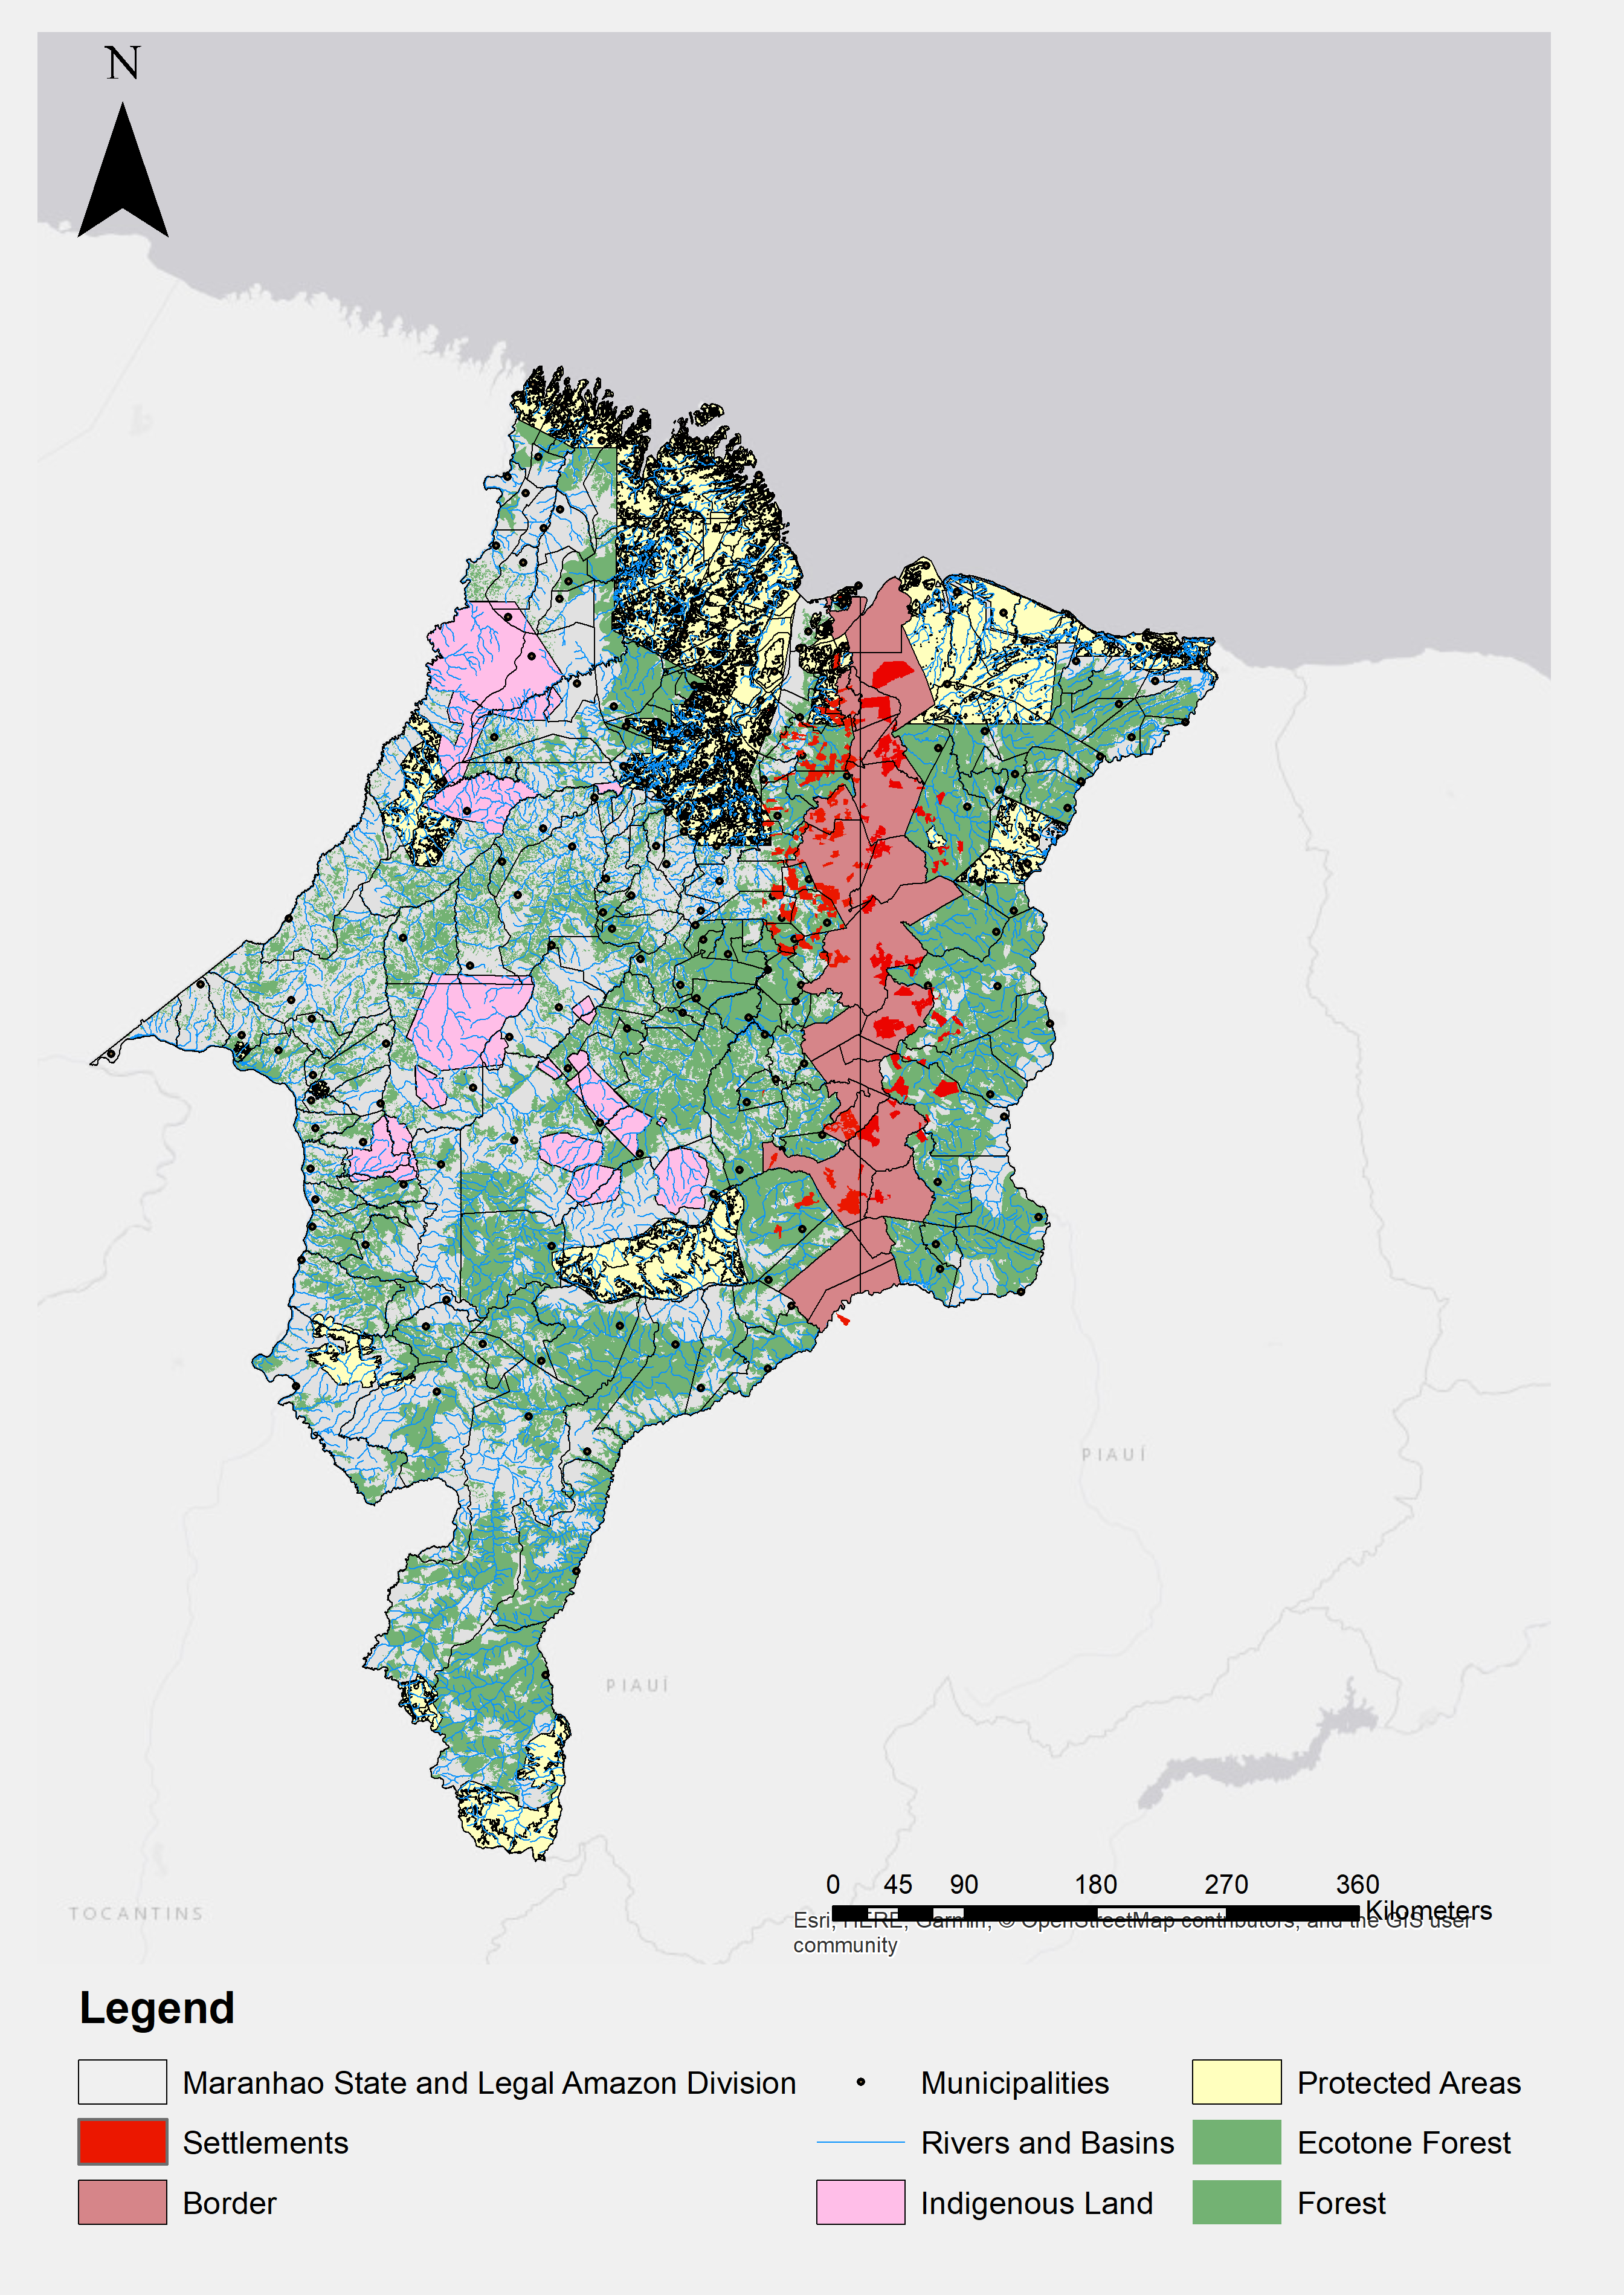
\includegraphics[width=1\textwidth, inner]{Chapter3/MaranhaoChapter3_Fig2.png}
\caption[Maranhão  state and settlements]{Maranhão  state and settlements within the studied municipalities. Source: \citep{MMMAwebsite,nugeo_2018}.}
\label{fig:delimitacaosett}
\end{figure}

The Kaplan Meier fitter shows that from the 37,532 pixels, in 2001, about 55\% of pixels had a chance of survival considering both vegetation indices. For 2010, the chance of survival decreased to the range of 5.8\% to 6.1\%. At the end of the studied period, the chance of survival for pixels within settlements were around 0.4\% and 0.6\% (see upper and bottom left graph from Figure \ref{fig:km-total-sett}). The median time of survival for the model was two years. This means that the half life of the sample pixels was around two years (the the 50th percentile). Sub-setting the survival curves by region, it's possible to identify that pixels within Legal Maranhão (LM) had a higher rate of survival comparing to pixels within Cerrado Maranhão (MA). The presence of clouds in this subset still shows that the chance of survival was higher in the Legal Maranhão (not shown). 

We performed a Log Rank test \citep{Peto_1972} to check whether the two sub samples were originated from the same distribution and the differences from these survival curves are produced from other characteristics than the region. The results suggested that these sub samples came from the same distribution which cannot reject the null hypothesis. However, given that the majority of the settlement pixels are deforested within two years, we also applied the generalized Wilcoxon test, which can be also referred to Log Rank Weighted test, because it gives more weight to early deforestation than later deforestation, while a Log Rank test gives equal weight to all deforestation process \citep{lee_wang_2003}. From the Log Rank Weighted test, at 5\% level, the two sub samples actually come from different distribution.


\begin{figure}[H]
  \centering
  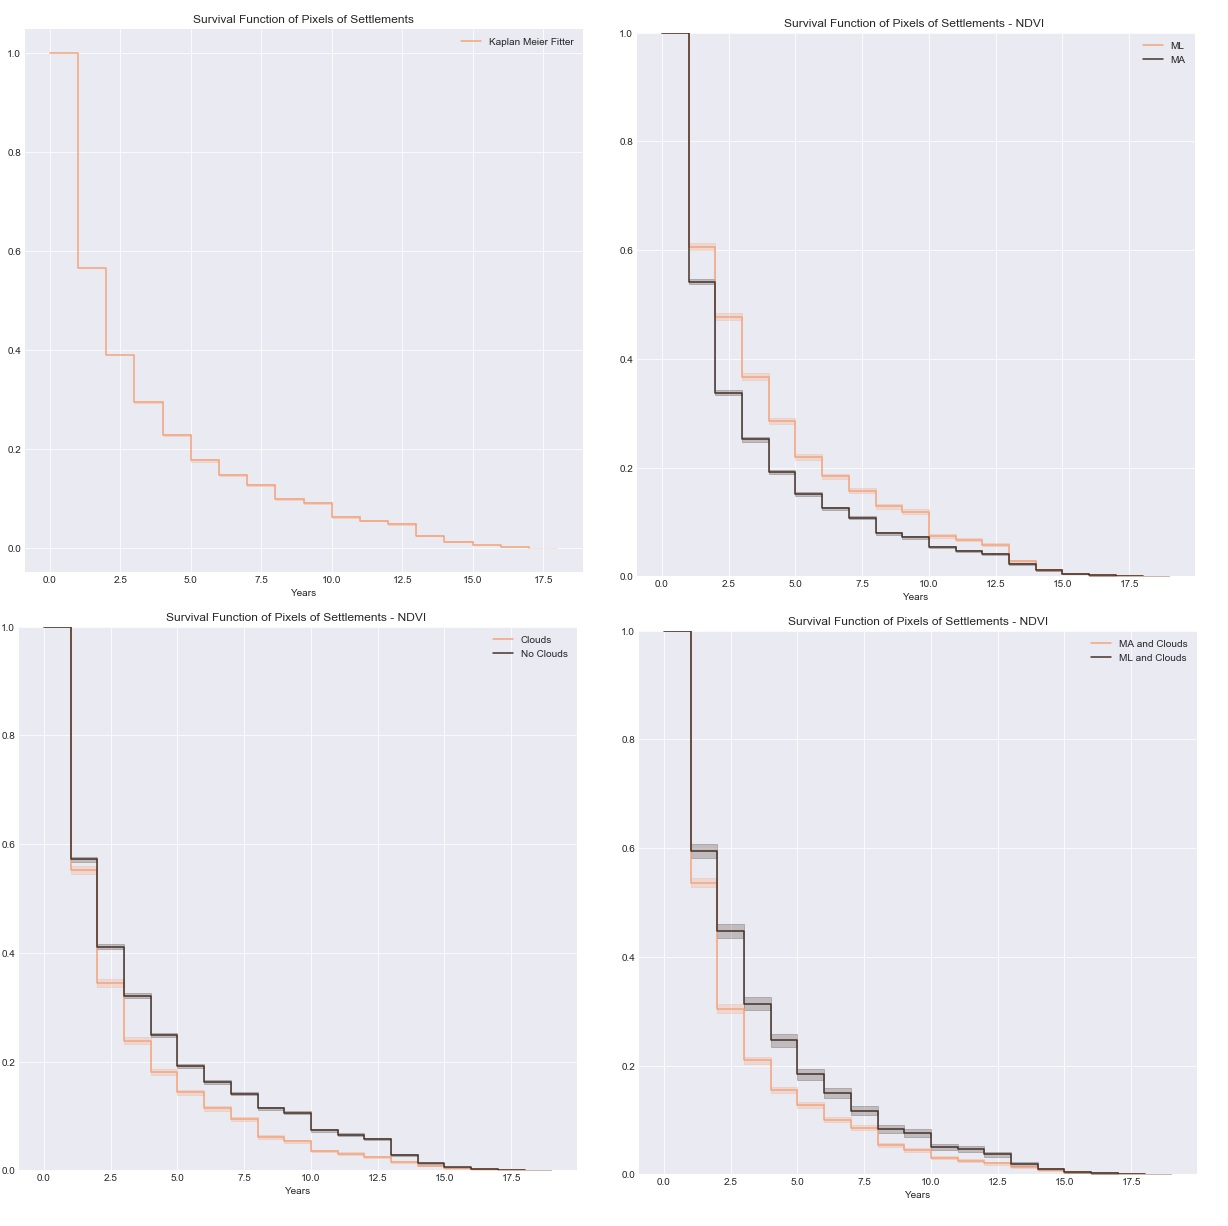
\includegraphics[width=1\textwidth]{KM_NDVI_sett_total.jpg}
\caption[Kaplan Meier Fitter for NDVI values in Settlements]{Kaplan Meier Fitter for NDVI values in the Settlements areas of Cerrado Maranhão  (MA) and Legal Maranhão  (LM). Top left shows the KM fitter for the Region and, at the top right, the stratified KM fitter of the Region. Bottom left shows the KM fitter for the Region stratifying by cloud coverage. At the bottom right, it shows the KM fitter stratifying by Clouds and Region.}
\label{fig:km-total-sett}
\end{figure}

%Cox time fitter
The results from the proportional hazard model is shown in Table \ref{tab:CPH_NDVI_sett}. The presence of clouds decreases hazard by 5\%. Elevation has a constant relative hazard. Distancing from municipalities centre decreases hazard by almost 27\%. Forested pixels within settlements and under the monitored policy area has a decreasing risk of being deforested comparing to non monitored areas. However, the presence of clouds in settlements located in the Legal Maranhão side increases the hazard by 4.2\%.

%Cox time fitter
The results from the proportional hazard model are shown in Table \ref{tab:CPH_NDVI_sett}. The presence of clouds decreases the hazard by 5\%. Elevation has a constant relative hazard. Distancing from municipalities centre decreases hazard by almost 27\%. Forested pixels within settlements and under the monitored policy area hves a decreasing risk of being deforested comparing to non monitored areas. However, the presence of clouds in settlements located in the Legal Maranhão side increases the hazard by 4.2\%, as can be seen from the coefficient on the interaction term between our regional dummy and cloud variable.

\begin{table}[H]
\footnotesize
\caption{Cox Proportional Hazard Model - Settlements}
\begin{tabularx}{\linewidth}{X YYYYY}
\hline
\hline
Variables	&	Regression Coefficient	&	Relative Hazards	&	Standard Errors	&	z score & Pr (>|z|) \\
\hline
Clouds	&	-0.052	&	0.950	&	0.014	&	-3.778	&	2E-04	***		\\
Pas	&	-0.011	&	0.989	&	0.045	&	-0.241	&	0.809			\\
Mining	&	-0.419	&	0.658	&	0.085	&	-4.933	&	8E-07	***		\\
Elevation	&	0.000	&	1.000	&	0.000	&	3.309	&	0.001	***		\\
Markets	&	0.026	&	1.027	&	0.029	&	0.903	&	0.366			\\
Municipalities	&	-0.306	&	0.737	&	0.084	&	-3.654	&	3E-04	***		\\
Rivers	&	1.431	&	4.183	&	0.345	&	4.148	&	3E-05	***		\\
Roads	&	0.234	&	1.264	&	0.139	&	1.685	&	0.092	.		\\
Lat	&	-0.154	&	0.857	&	0.018	&	-8.76	&	<	2E-16	***	\\
Lon	&	0.332	&	1.393	&	0.048	&	6.944	&	4E-12	***		\\
Region	&	-0.079	&	0.924	&	0.022	&	-3.525	&	4E-04	***		\\
Clouds*Region	&	0.041	&	1.042	&	0.021	&	1.995	&	0.046	*		\\
\hline
\hline
\multicolumn{6}{l}{Signs stand for '***' 0.001 '**' 0.01 '*' 0.05 '.' 0.1 and denote hazard ratios that are significantly}\\
\multicolumn{6}{l}{ different from 1 at 99\%, 95\% and 90\% confidence levels. The model contains controls for grouped year}\\
\multicolumn{6}{l}{periods. PAs stand for Protected Areas. Indigenous Lands and Conservational Units.}\\
\end{tabularx}%
\label{tab:CPH_NDVI_sett}%
\end{table}%

A likelihood ratio test again suggested that it was better to divide the sample area according to the region. The results are presented in Tables \ref{tab:CPH_NDVI_sett_MA} and \ref{tab:CPH_NDVI_sett_ML}. For the non surveilled area, the presence of clouds decreased hazard by almost 4\%. Also increasing the distance to protected areas and mining centres by one degree decreases the hazard by 56\% and 50\%, respectively. For the Legal Maranhão side, the presence of clouds has no effect on the relative hazard. Differently from the neighbouring area, distancing from protected areas and mining centres increase hazard by 38\% and 76\%. Distancing from urban and market areas has a negative impact on the hazard. For markets the relative hazard decreases by 10\% and for municipalities centre the amount decreased is almost 56\%. 

\begin{table}[H]
\footnotesize
\caption{Cox Proportional Hazard Model - Settlements (MA)}
\begin{tabularx}{\linewidth}{X YYYYY}
\hline
Variables	&	Regression Coefficient	&	Relative Hazards	&	Standard Errors	&	z score & Pr (>|z|) \\
\hline
\hline
Clouds	&	-0.038	&	0.963	&	0.014	&	-2.665	&	0.008	**		\\
PAs	&	-0.626	&	0.535	&	0.081	&	-7.69	&	0.000	***		\\
Mining	&	-0.684	&	0.504	&	0.100	&	-6.855	&	0.000	***		\\
Elevation	&	0.000	&	1.000	&	0.000	&	-0.915	&	0.360			\\
Markets	&	0.535	&	1.708	&	0.057	&	9.469	&	<	2E-16	***	\\
Municipalities	&	-0.358	&	0.699	&	0.108	&	-3.328	&	0.001	***		\\
Rivers	&	0.997	&	2.711	&	0.448	&	2.228	&	0.026	*		\\
Roads	&	0.266	&	1.305	&	0.156	&	1.702	&	0.089	.		\\
Lat	&	0.043	&	1.044	&	0.030	&	1.452	&	0.147			\\
Lon	&	0.446	&	1.562	&	0.060	&	7.407	&	0.000	***		\\
\bottomrule
\multicolumn{6}{l}{Signs stand for '***' 0.001 '**' 0.01 '*' 0.05 '.' 0.1 and denote hazard ratios that are significantly}\\
\multicolumn{6}{l}{ different from 1 at 99\%, 95\% and 90\% confidence levels. The model contains controls for grouped year}\\
\multicolumn{6}{l}{periods. PAs stand for Protected Areas. Indigenous Lands and Conservational Units.}\\
\end{tabularx}%
\label{tab:CPH_NDVI_sett_MA}%
\end{table}%


\begin{table}[H]
\footnotesize
\caption{Cox Proportional Hazard Model - Settlements (LM)}
\begin{tabularx}{\linewidth}{X YYYYY}
\hline
Variables	&	Regression Coefficient	&	Relative Hazards	&	Standard Errors	&	z score & Pr (>|z|) \\
\hline
\hline
Clouds	&	0.006	&	1.006	&	0.017	&	0.340	&	0.734			\\
PAs	&	0.323	&	1.382	&	0.084	&	3.849	&	0.000	***		\\
Mining	&	0.567	&	1.762	&	0.222	&	2.558	&	0.011	*		\\
Elevation	&	0.001	&	1.001	&	0.000	&	3.616	&	0.000	***		\\
Markets	&	-0.097	&	0.907	&	0.049	&	-1.976	&	0.048	*		\\
Municipalities	&	-0.615	&	0.541	&	0.170	&	-3.614	&	0.000	***		\\
Rivers	&	1.377	&	3.963	&	0.581	&	2.372	&	0.018	*		\\
Roads	&	-0.543	&	0.581	&	0.345	&	-1.573	&	0.116			\\
Lat	&	-0.236	&	0.790	&	0.028	&	-8.442	&	<	2E-16	***	\\
Lon	&	0.471	&	1.602	&	0.110	&	4.300	&	2E-05	***		\\
\bottomrule
\multicolumn{6}{l}{Signs stand for '***' 0.001 '**' 0.01 '*' 0.05 '.' 0.1 and denote hazard ratios that are significantly}\\
\multicolumn{6}{l}{ different from 1 at 99\%, 95\% and 90\% confidence levels. The model contains controls for grouped year}\\
\multicolumn{6}{l}{periods. PAs stand for Protected Areas. Indigenous Lands and Conservational Units.}\\
\end{tabularx}%
\label{tab:CPH_NDVI_sett_ML}%
\end{table}%

The extended Cox model presented in equation \ref{eq:8} is also applied to the settlements. Accordingly, the presence of clouds has no effect in the presence of the relative hazard. In contrast, a one unit greater distance from protected areas and mines increase the relative hazard by 12\% and 22\% , as can be seen from Table \ref{tab:CPH_NDVI_sett_time}. Municipalities centre are not significant in the model. The relative hazard decreases 80\% if the pixels are far from markets. Rivers and roads have no impact on relative hazard. The incidence of clouds in settlement pixels within the Legal Maranhão also has no impact on the relative hazard. Increasing the level of rain decreases the hazard by 0.01\%. Even though an increasing the level of temperature increases the relative risk of a pixel being deforested, increasing the temperature in the Legal Maranhão decreases the hazard by almost 3\%. 

The analysis for the two regions separated suggests similar patterns. Clouds have no effect on the relative hazard. In contrast, neighbouring forested areas increase the hazard by 15\% in the Legal Maranhão, and twice the relative hazard in the Cerrado Maranhão. Increasing rainfall levels will decrease the hazard in both sides by approximately 2\%, while higher levels of temperature increase hazard in both regions ranging from 1 to 5\%. 

\begin{table}[H]
\footnotesize
\caption{Cox Proportional Hazard Model Time Dependent - Settlements}
\begin{tabularx}{\linewidth}{X YYYYY}
\hline
\hline
Variables	&	Regression Coefficient	&	Relative Hazards	&	Standard Errors	&	z score & Pr (>|z|) \\
\hline
Clouds	&	0.031	&	1.032	&	0.020	&	1.535	&	0.125		\\
PAs	&	0.116	&	1.123	&	0.066	&	1.766	&	0.077	.	\\
Mining	&	0.573	&	1.774	&	0.111	&	5.162	&	2E-07	***	\\
Elevation	&	0.000	&	1.000	&	0.000	&	2.376	&	0.018	*	\\
Markets	&	-0.218	&	0.804	&	0.042	&	-5.232	&	2E-07	***	\\
Municipalities	&	0.067	&	1.069	&	0.115	&	0.582	&	0.561		\\
Rivers	&	0.873 &	2.393 &	0.735 &	1.188 &	0.235	\\
Roads	&	-0.293	&	0.746	&	0.191	&	-1.53	&	0.126		\\
Lat &	-0.106	&	0.900	&	0.026	&	-4.074	&	5E-05	***	\\
Lon	&	0.016	&	1.016	&	0.057	&	0.288	&	0.773		\\
Region	&	0.573	&	1.773	&	0.111	&	5.162	&	2E-07	***	\\
Clouds*Region	&	-0.028	&	0.972	&	0.028	&	-0.99	&	0.322		\\
Neighbours	&	0.317	&	1.373	&	0.111	&	2.863	&	0.004	**	\\
Rainfall	&	-0.003	&	0.997	&	0.001	&	-5.331	&	1E-07	***	\\
Rainfall*Region	&	0.001	&	1.001	&	0.001	&	0.859	&	0.390		\\
Temperature	&	0.025	&	1.025	&	0.004	&	6.855	&	7E-12	***	\\
Temperature*Region	&	-0.021	&	0.979	&	0.004	&	-5.476	&	4E-08	***	\\
\hline
\hline
\multicolumn{6}{l}{Signs stand for '***' 0.001 '**' 0.01 '*' 0.05 '.' 0.1 and denote hazard ratios that are significantly }\\
\multicolumn{6}{l}{different from 1 at 99\%, 95\% and 90\% confidence levels. The model contains controls for grouped and }\\
\multicolumn{6}{l}{time-dependent year periods. PAs stand for Protected Areas. Indigenous Lands and Conservational Units.}\\
\end{tabularx}%
\label{tab:CPH_NDVI_sett_time}%
\end{table}%

Finally, with the settlements analysis, it is likely that the environmental policy could not detain deforestation during the last two decades in the ecotonic region of Maranhão. According to the results, the forests inside the surveillance area had a lower probability of survival comparing to the area not covered by the policy. The presence of clouds along with climatic variables was an active barrier to the legal compliance and, since the studied area has no systematic differences, we can agree on the lack of effectiveness due to cloud barrier. Since these barrier indicate different form of seasonality, the probability of a pixel being deforested in the rainy season is higher comparing to dry season which in turn evidence the behaviour change. We deduce that our results justify the undermining effect of the environmental policy caused by the changing behaviour and the presence of the artificial line.

\section{Conclusions}
\label{S:6}


In this study we quantified the effect of cloud coverage, which inhibits satellite detection of disturbances to local forest, on local levels of deforestation in the Brazilian Amazon. To this end we focused on the ecological tension zone of Maranhão because it is divided by an artificial line that separates it in two  parts, one for which there is satellite monitoring (the Legal Amazon Maranhão)  and one (Cerrado Maranhão) for which no such monitoring was in place.  Thus arguably the role of cloud coverage in local forest losses should be different across this synthetic border.  Identification of local deforestation was done through an algorithm to capture Vegetation Indices changes over time using satellite images.  Similarlly satellite images were used to detect corresponding local cloud coverage.  To estimate the impact of the latter on the former we employed a survival analysis on homogenously forested regions near the border. Our results showed that clouds indeed played an important role in encouraging deforestation on the side that is under the satellite monitoring program, while they were not determinants of forest loss in cells across the border. This was further supported by examining settlement areas on both sides of the border where there was also no satellite detection in place.  This strongly suggests that clouds inhibited the detection process of the satellite monitoring program in place.   

%In the results, we conclude that protected areas and roads are a great risk to the survival of forests. Protected areas reflect the action of past deforestation and then, the pressure on these special zones is transitioned to their borders. Roads indicate infrastructure expansion and is usually considered a proximate driver. Our findings explain that forests close to roads has a higher chance of being cleared. Mainly, forested pixels covered by clouds in the surveillance area has a higher chance of being deforested than in the not monitored area. Having forested pixels nearby increases the chance of being deforested which is assimilating the anthropic pressure on the environment. Finally, rainfall and temperature also affects the hazard. For the environmentally regulated region, intensive showers and lower temperatures increase the probability of a forested pixel being deforested. For the non regulated side, rainfall and lower temperature decreases the aforementioned probability.

We acknowledge a number of limitations to the resulted analysis. Firstly, the model implicitly assumes that in the first year of the study all pixels were fully occupied by forest, which in reality might not be true. It is also possible that the spatial distribution of the vegetation indices may exhibit dynamic behaviour over time, so that a potential area may or may not be sparsely vegetated for a certain period (e.g., during sampling) due to progressive succession of attacks of pests and diseases, which could not be distinguished from true permanent deforestation by the vegetation indices. Secondly, the study was based on  coarse image resolution which could neglect local changes (< 250m) in the sample area. Thirdly, our results may not be generalised to other areas, such as dense tropical forests and sparse open fields. In addition, we only considered for the analysis covariates existent before or from 2000, which thus excluded roads, protected areas, indigenous land, markets, municipalities centre, and, mining/mineral resources created or discovered after 2000. Finally, we acknowledge that the models were derived from NDVI values and that one could alternatively have used EVI values, which in some instances might be more suited for ecotone forests \citep{ratana_huete_ferreira_2005,bayma_sano_2015,didan_munoz_2015}.

\let\cleardoublepage\clearpage
\begin{appendices} \label{appendix}
\renewcommand{\thechapter}{A.\arabic{chapter}}
%!TEX root = ../chapter3.tex
% ******************************* Thesis Appendix A ****************************

\chapter{}

\begin{sidewaystable}
\begin{figure}[H]
  \centering
  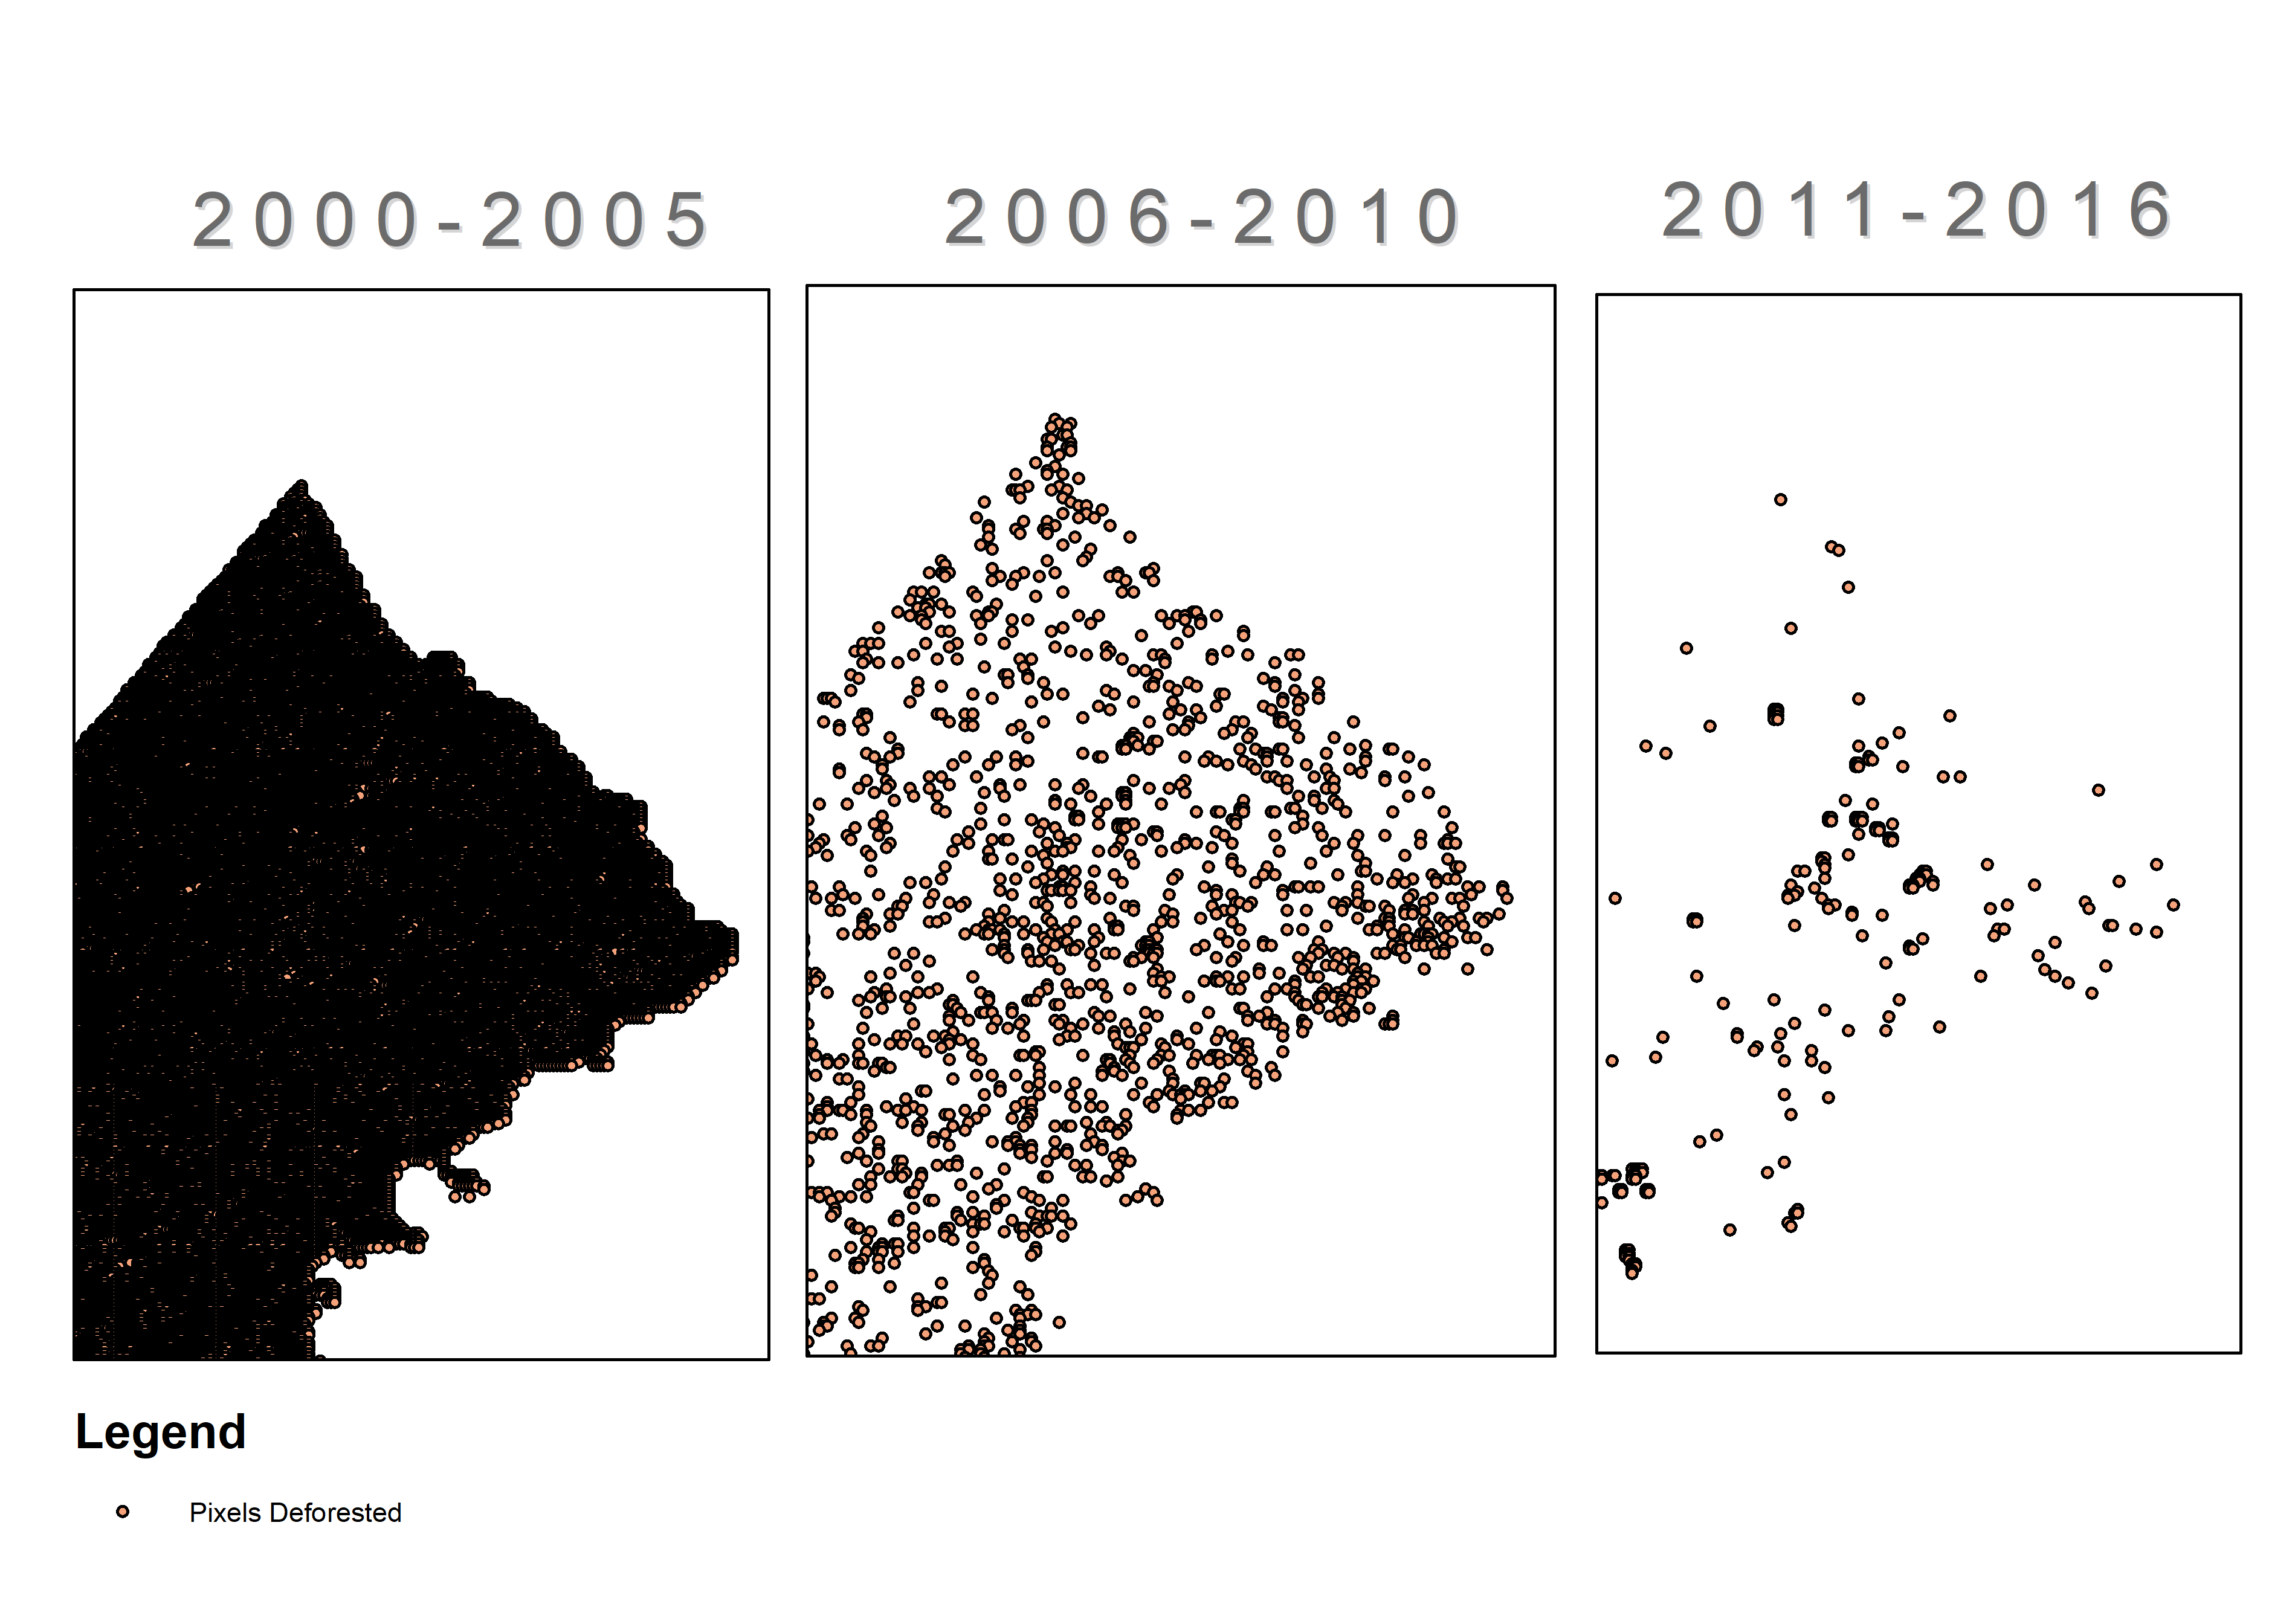
\includegraphics[width=0.85\textwidth]{Chapter3/ML_pixels_death.png}
\caption[Remaining Pixels in Legal Maranhão side]{Remaining Pixels in Legal Maranhão side for three different year periods. Pixels are only counted once. Area was randomly chosen.}
\label{fig:remainingLM}
\end{figure}
\end{sidewaystable}

\begin{sidewaystable}
\begin{figure}[H]
  \centering
  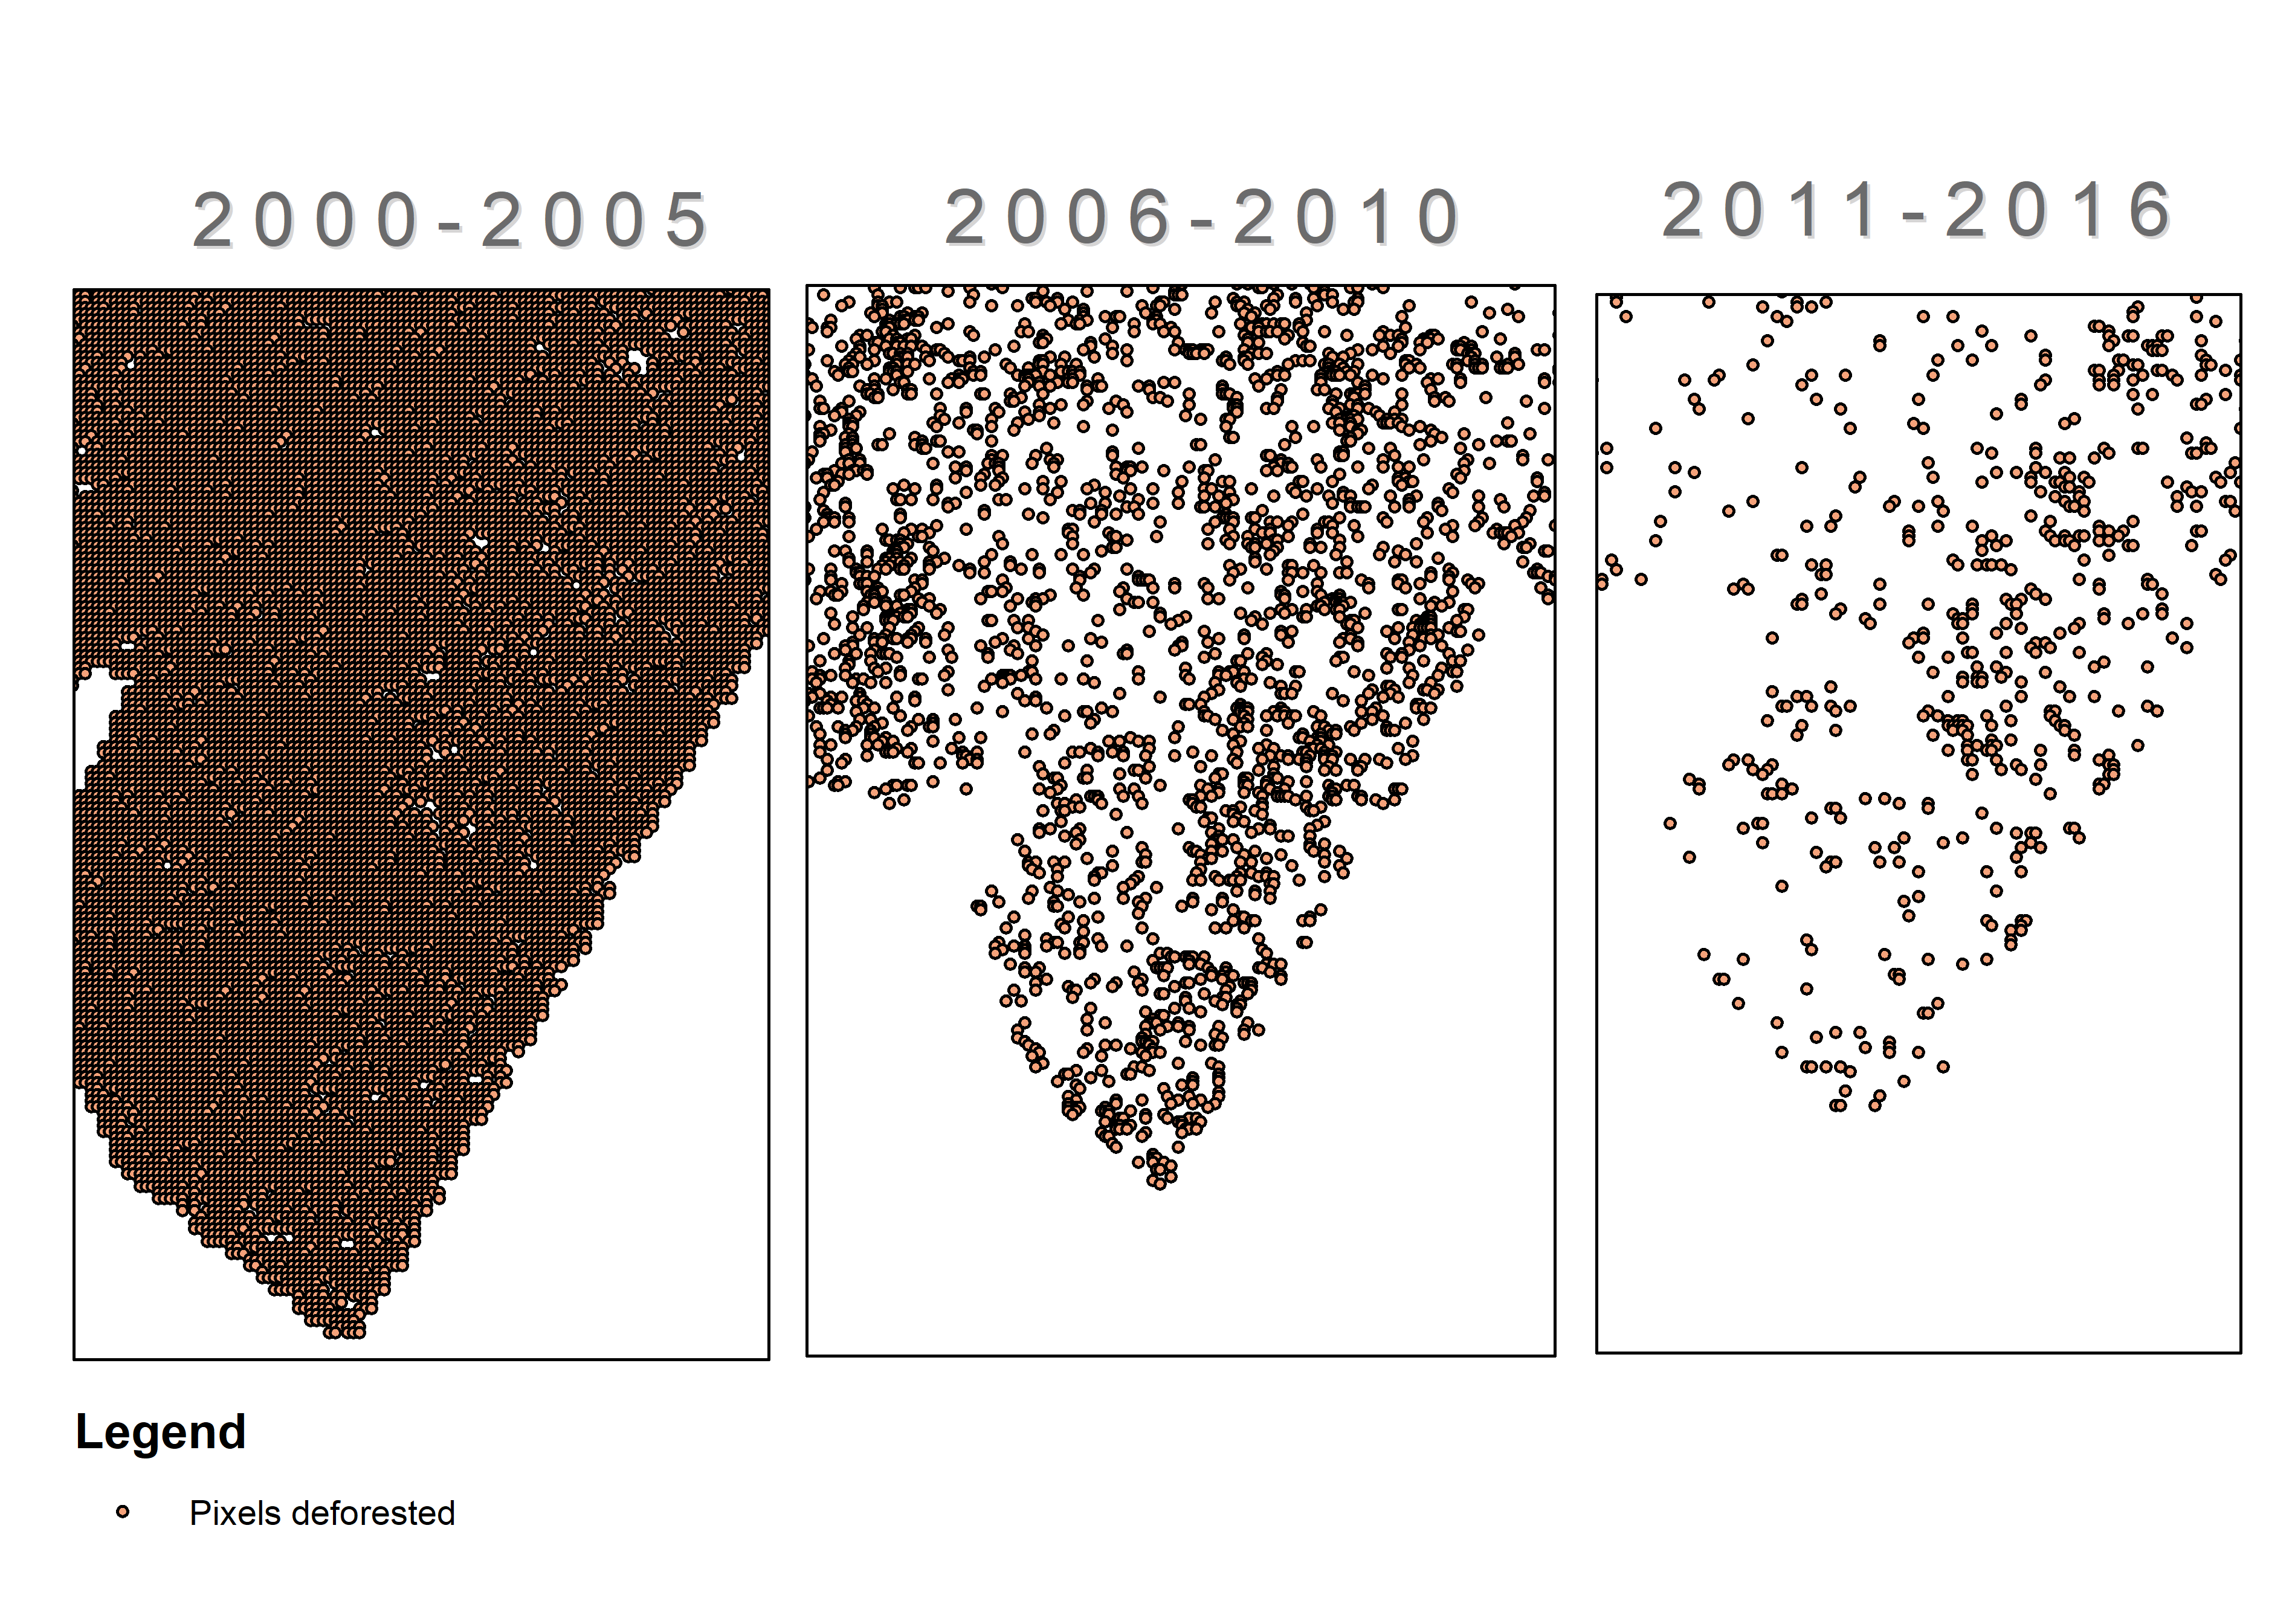
\includegraphics[width=0.85\textwidth]{Chapter3/MA_pixels_death.png}
\caption[Remaining Pixels in Cerrado Maranhão side]{Remaining Pixels in Cerrado Maranhão side for three different year periods. Pixels are only counted once. Area was randomly chosen.}
\label{fig:remainingMA}
\end{figure}
\end{sidewaystable}

\begin{sidewaystable}
\begin{figure}[H]
  \centering
  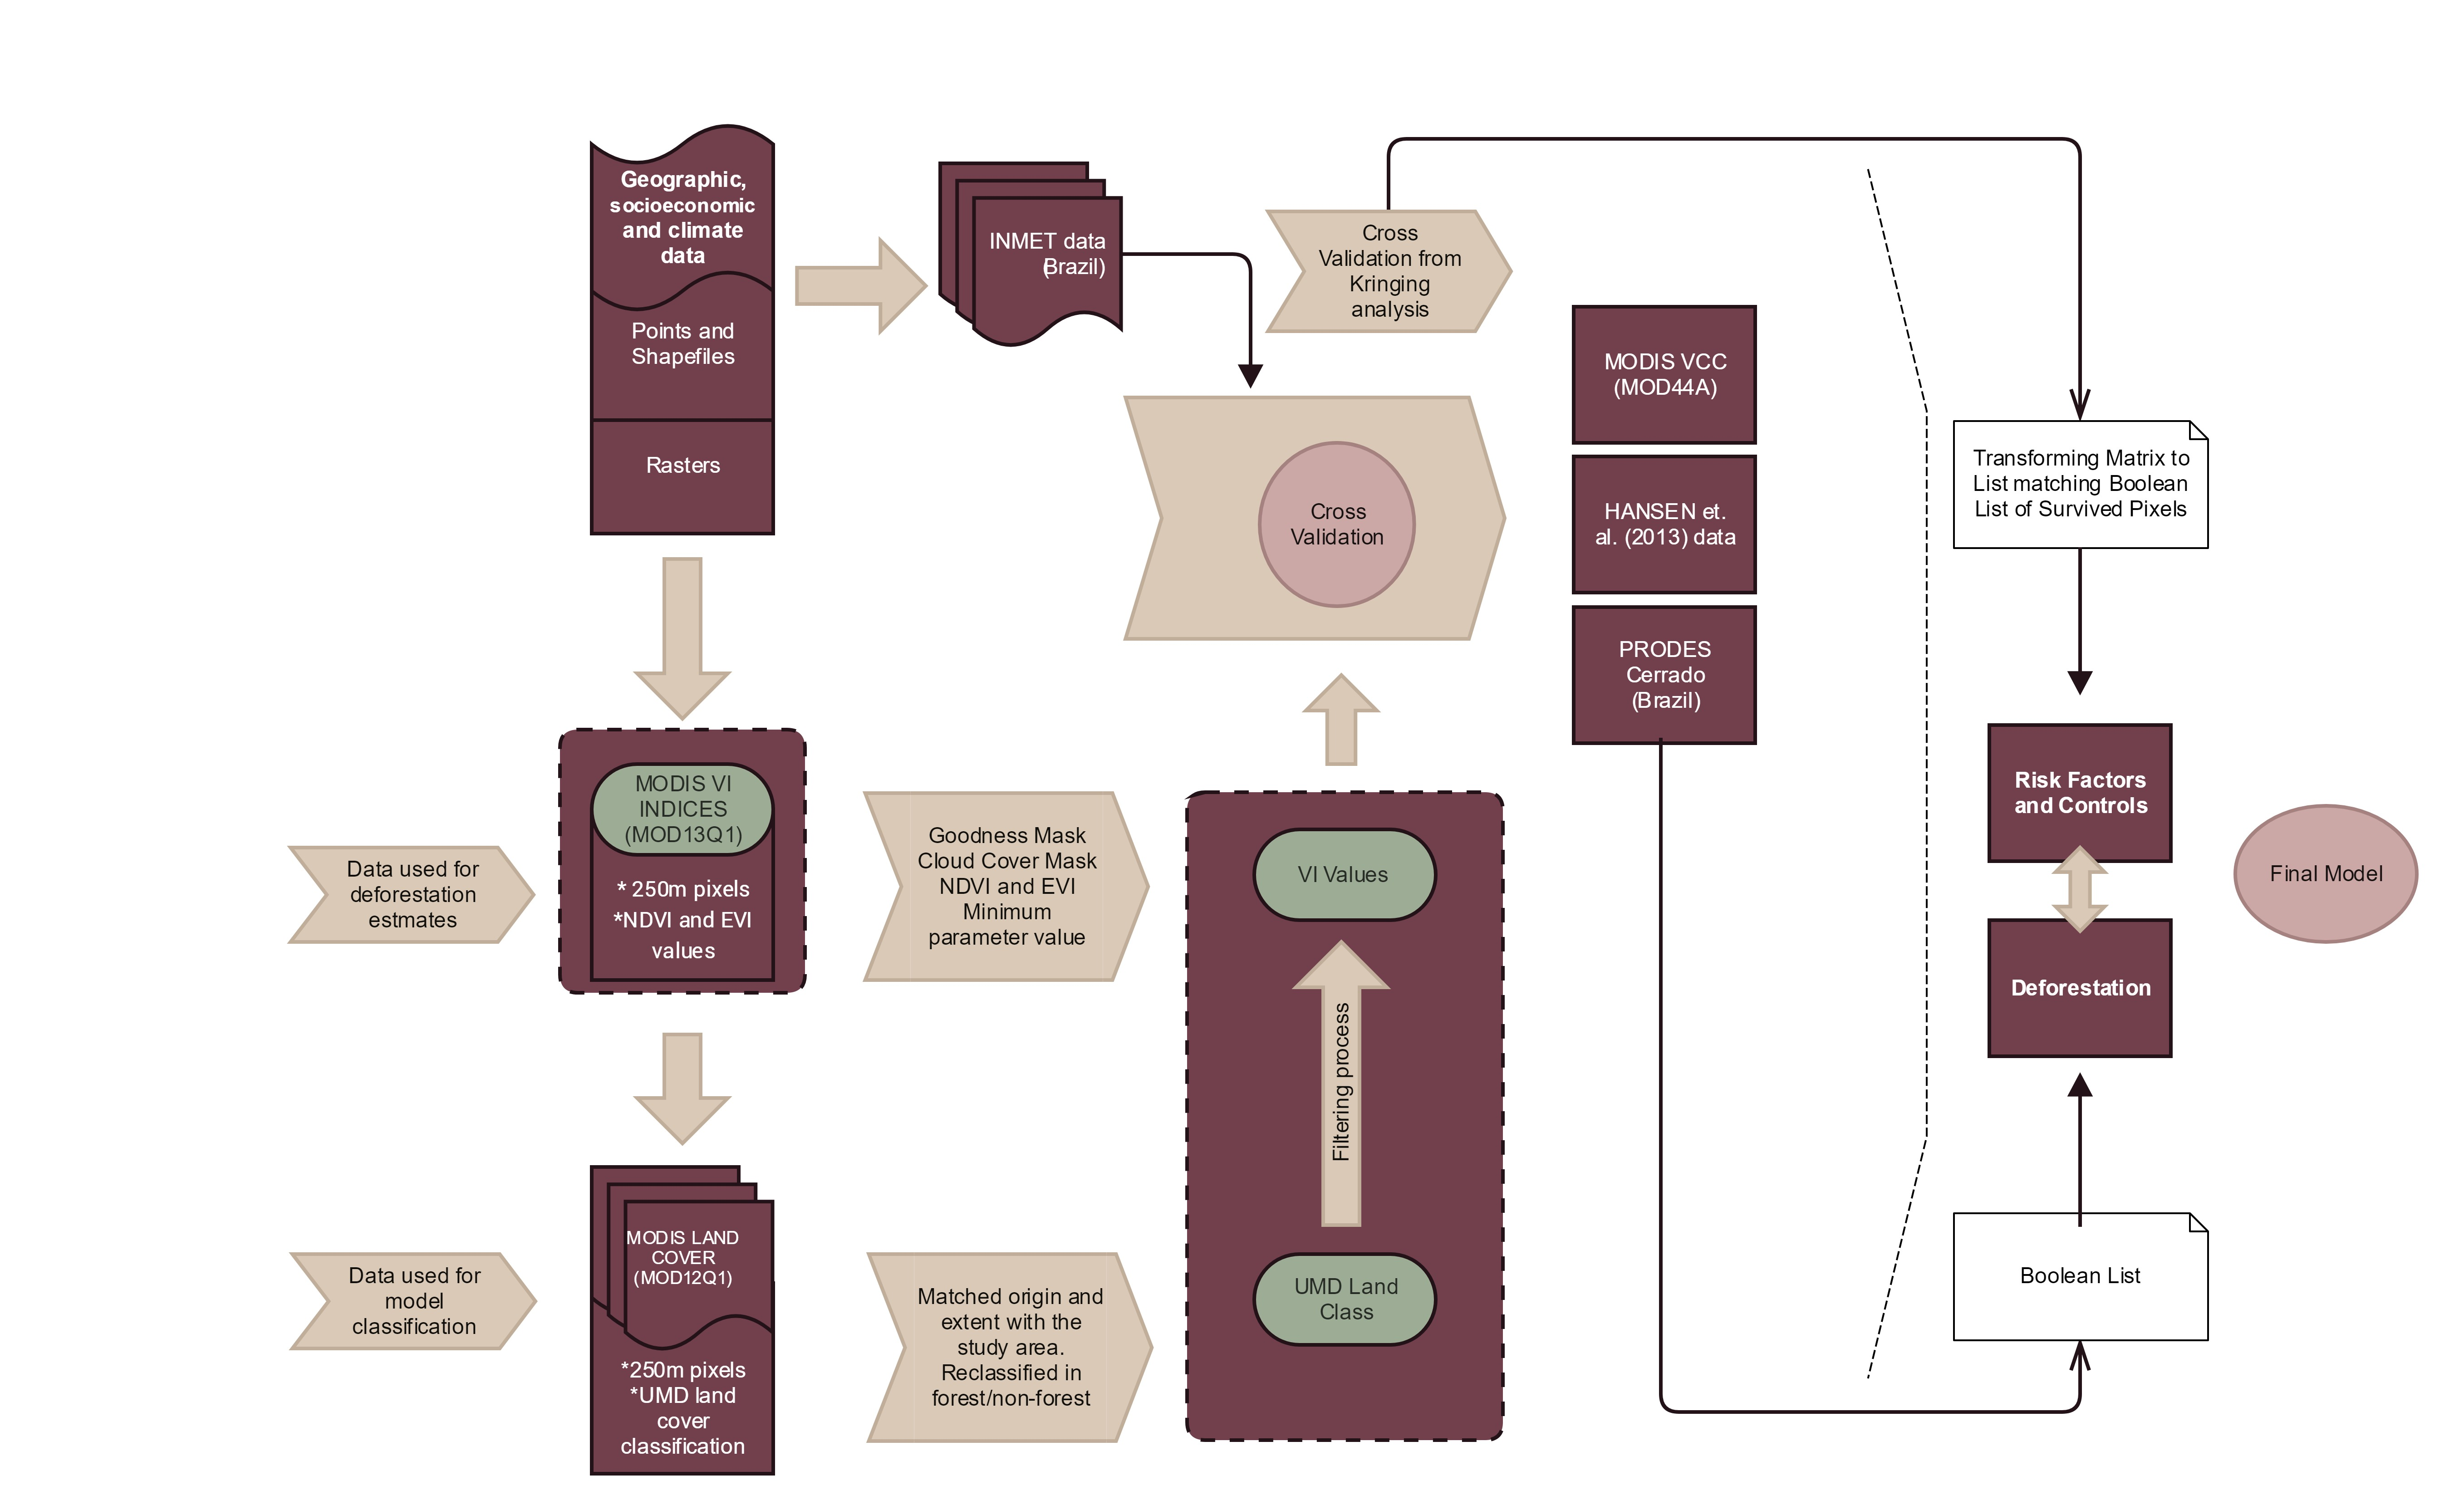
\includegraphics[width=9\textwidth]{method.jpg}
\caption[Flowchart of method applied to data]{Flowchart of method applied to data. Moving from left to right indicates increasing levels of data processing during the study.}
\label{fig:method}
\end{figure}
\end{sidewaystable}

\begin{table}[H]
\footnotesize
\caption{Model Selection and Validation}
\begin{tabularx}{\linewidth}{X CCCC}
\hline
\hline
Models	& Concordance index & Std Deviation &	K-fold (k=3)	&	Std Deviation \\
\hline
NDVI MA	& 0.767 & 0.001 &	0.30	&	0.0004 \\
NDVI ML	& 0.691 & 0.001	& 0.69	&	0.0008 \\
NDVI Region & 0.755 & 0.001	&	0.03	&	0.0004 \\
EVI MA	& 0.735 & 0.001	& 0.39	&	0.0011 \\
EVI ML & 0.691 & 0.001	&	0.69	&	0.0008 \\
EVI Region & 0.732 & 0.001	&	0.08	&	0.0008 \\
NDVI Sett MA & 0.780 & 0.003 &	0.77	&	0.0040 \\
NDVI Sett ML & 0.798 & 0.003 &	0.79	&	0.0019 \\
NDVI Sett Region & 0.785 & 0.002 &	0.78	&	0.0013 \\
NDVI Buffer MA & 0.582 & 0.005	&	0.58	&	0.0066 \\
NDVI Buffer ML & 0.689 & 0.003	&	0.68	&	0.0052 \\
NDVI Buffer Region & 0.668 & 0.003	&	0.66	&	0.0003 \\
\hline
\hline
\multicolumn{5}{l}{\footnotesize Concordance Index is computed along with the statistical results. K-fold validation is computed using the} \\
\multicolumn{5}{l}{\footnotesize results from the statistical analysis as input for the calculation.}
\end{tabularx}
\label{kfold}
\end{table}

\begin{table}[H]
\footnotesize
\caption{Descriptive Statistics - Vegetation Indices (Region)}
\begin{tabularx}{\linewidth}{X CCCC}
\hline
\hline
Variables	&	Mean	&	Std Deviation	&	Min	&	Max	 \\
\hline
Period (N)	&	2.653	&	2.628	&	0.000	&	17.000	\\
Censored (N)	&	0.967	&	0.180	&	0.000	&	1.000	\\
Cloud (N)	&	0.711	&	0.453	&	0.000	&	1.000	\\
Period (E)	&	2.459	&	2.344	&	0.000	&	17.000	\\
Censored (E)	&	0.967	&	0.180	&	0.000	&	1.000	\\
Cloud (E)	&	0.711	&	0.453	&	0.000	&	1.000	\\
Lat	&	-2.683	&	0.223	&	-3.064	&	-2.347	\\
Lon	&	-41.892	&	1.171	&	-44.601	&	-39.584	\\
PAs	&	0.539	&	0.355	&	0.000	&	1.228	\\
Mining	&	0.053	&	0.085	&	0.000	&	0.461	\\
Elevation	&	137.934	&	100.009	&	-26	&	993 \\
Markets	&	0.502	&	0.235	&	0.000	&	1.095	\\
Municipalities &	0.128	&	0.058	&	0.000	&	0.341	\\
Rivers	&	0.017	&	0.015	&	0.000	&	0.211	\\
Roads	&	0.037	&	0.037	&	0.000	&	0.218	\\
Region	&	0.404	&	0.491	&	0.000	&	1.000	\\
Neighbours  & 0.992 & 0.161 & 0.000 & 1.000 \\
Rainfall & 130 & 35.695 & 0.000 & 214 \\
Temperature  & 31.7 & 6.241 & 29 & 34 \\
\hline
\hline
\multicolumn{5}{l}{\footnotesize Statistics refer to N=529,680 pixels observations. (N) refers to NDVI and (E) refers to EVI. All distancing }\\
\multicolumn{5}{l}{\footnotesize  values are in decimal degrees. The conversion assumes 0.1 degree to 11km$^{2}$.}
\end{tabularx}
\label{tab:summary}
\end{table}

\begin{table}[H]
\footnotesize
\caption{Descriptive Statistics - Vegetation Indices (MA and LM)}
\begin{tabularx}{\linewidth}{X CCCC}
\hline
\hline
Variables (MA)	&	Mean	&	Std Deviation	&	Min	&	Max	 \\
\hline
Period (N)	&	3.059	&	3.053	&	0.000	&	17.000	\\
Censoring (N)	&	0.956	&	0.205	&	0.000	&	1.000	\\
Clouds (N)	&	0.517	&	0.500	&	0.000	&	1.000	\\
Lat	&	-2.527	&	0.119	&	-2.974	&	-2.347	\\
Lon	&	-41.820	&	1.174	&	-43.980	&	-39.584	\\
Pas	&	0.512	&	0.388	&	0.000	&	1.228	\\
Mining	&	0.065	&	0.098	&	0.000	&	0.461	\\
Elevation	&	123.893	&	87.687	&	-26.000	&	993.000	\\
Markets	&	0.499	&	0.172	&	0.111	&	0.968	\\
Municipalities	&	0.130	&	0.060	&	0.000	&	0.341	\\
Rivers	&	0.017	&	0.016	&	0.000	&	0.211	\\
Roads	&	0.042	&	0.040	&	0.000	&	0.218	\\
Neighbours  & 0.995 &	0.049 &	0.000 &	1.000 \\
Rainfall & 138.9 & 24.877 & 0.000 & 203.000 \\
Temperature  & 32.845 & 1.448 & 29.000 & 34.000 \\
\hline
Variables (LM)	&	Mean	&	Std Deviation	&	Min	&	Max	 \\
\hline
Period (N)	&	2.091	&	1.643	&	0.000	&	17.000	\\
Censoring (N)	&	0.486	&	0.500	&	0.000	&	1.000	\\
Clouds (N)	&	0.941	&	0.235	&	0.000	&	1.000	\\
Lat	&	-2.896	&	0.139	&	-3.064	&	-2.347	\\
Lon	&	-41.987	&	1.134	&	-44.599	&	-39.603	\\
Pas	&	0.580	&	0.310	&	0.000	&	1.227	\\
Mining	&	0.037	&	0.065	&	0.000	&	0.461	\\
Elevation	&	1.542	&	1.094	&	-0.030	&	4.940	\\
Markets	&	0.509	&	0.291	&	0.000	&	1.095	\\
Municipalities	&	0.129	&	0.058	&	0.000	&	0.341	\\
Rivers	&	0.016	&	0.013	&	0.000	&	0.079	\\
Roads	&	0.032	&	0.031	&	0.000	&	0.211	\\
Neighbours	&	0.991	&	0.066	&	0.000	&	1.000	\\
Rainfall	&	116.867	&	44.567	&	0.000	&	214.000	\\
Temperature	&	30.011	&	9.522	&	29.000	&	34.000	\\
\hline
\hline
\multicolumn{5}{l}{\footnotesize Statistics refer to N=529,680 pixels observations. (N) refers to NDVI and (E) refers to EVI. All distancing }\\
\multicolumn{5}{l}{\footnotesize  values are in decimal degrees. The conversion assumes 0.1 degree to 11km$^{2}$.}
\end{tabularx}
\label{tab:summaryMALM}
\end{table}

\begin{sidewaystable}
\begin{table}[H]
\footnotesize
    \caption{Data Description - Sources}
       \begin{tabularx}{0.88\linewidth}{l CXCC}
     \hline
     \hline
       Variable & Source & Description  & Source Data Type & Source Resolution \\
     \hline
    Vegetation Indices & USGS/NASA & Vegetation Index (VI) value at a per pixel basis.  & Raster & 250m \\
    Land Cover & USGS/NASA  & Global land cover types at yearly intervals derived from six different classification schemes. & Raster & 500m\\
    Pas	& MMA & Euclidean distance to nearest protected area in decimal degrees & Polygon & - \\
    Mines & EMBRAPA & Euclidean distance to nearest mineral resource/mining in decimal degrees & Point & -\\
    Elevation & EMBRAPA & Digital elevated map of Maranhão & Raster & 30m\\
    Markets	& CONAB & Euclidean distance to nearest market in decimal degrees & Point & -\\
    Municipalities	& IBGE & Euclidean distance to nearest municipality centre in decimal degrees & Point & -\\
    Rivers	& IBGE & Euclidean distance to nearest river/basin in decimal degrees & Polyline & - \\
    Roads	& IBGE & Euclidean distance to nearest road in decimal degrees & Polyline & - \\
    Settlements & INCRA & Polygons of the settlement areas & Polygon & -\\
    Latitude and Longitude & IBGE & The latitude and longitude of each pixel in the study. This is used to account for spatial autocorrelation across large distances. & Raster & 250m \\
    \hline
    \hline
    \end{tabularx}%
 \label{tab:sources}%
\end{table}%
\end{sidewaystable}
\end{appendices}
 